% !TEX root = ../algo-summary.tex

\section{Complexity Theory}\label{sec:complexity_theory}

`efficiently solvable' = solvable in polynomial time.

many problems arre `hard', i.e. no known polynomial time solution is known

a large class of such problems has been characterized and shown to be equivalent:
NP-complete problems.
a polynomial algo for one would mean a polynomial time algo for \emph{all} NP-complete problems.

NP-complete in practice: prolems that are computationally hard for all partical purposes. 
look for an approximation algorithm.

\smallskip
{
\renewcommand{\arraystretch}{1.4}
\centering
\begin{tabular}{>{\raggedright\arraybackslash}p{0.4\linewidth} >{\raggedright\arraybackslash}p{0.45\linewidth}}
{\textcolor{AccentBlue}{Algorithm design patterns.}} & {\textcolor{AccentBlue}{Example}} \\
% \hline
Greed. & $O(n\log n)$ interval scheduling. \\
Divide-and-conquer. & $O(n\log n)$ FFT, merge sort. \\
Dynamic programming. & $O(n^{2})$ edit distance. \\
Duality. & $O(n^{3})$ bipartite matching. \\
\textcolor{AccentRed}{Reductions.} & \\ 
\textcolor{gray}{Local search.} & \\
\textcolor{gray}{Randomization.} & \\[2mm]
% \hline
{\textcolor{AccentBlue}{Algorithm design anti-patterns.}} & \\
% \hline
\textcolor{AccentRed}{NP-completeness.} & $O(n^k)$ algorithm unlikely. \\
PSPACE-completeness. & $O(n^k)$ certification algorithm unlikely. \\
Undecidability. & No algorithm possible. \\
\end{tabular}
}

\medskip

\textcolor{AccentBlue}{Working Definition} [Cobham 1964, Edmonds 1965, Rabin 1966].
In practice, we are able to solve problems with polynomial time algorithms.


Which problems will we be able to solve in practice?

\begin{tabular}{>{\raggedright\arraybackslash}p{0.34\linewidth} |>{\raggedright\arraybackslash}p{0.45\linewidth}}
{\textcolor{AccentBlue}{Yes}} & {\textcolor{AccentBlue}{Probably No}} \\
\hline
Shortest path & Longest path \\
Matching & 3D-matching \\
\nameref{prob:min_cut} & Max Cut \\
2-SAT & 3-SAT \\
Planar 4-color & Planar 3-color \\
Bipartite vertex cover & Vertex cover \\
Primality testing & Factoring \\
\end{tabular}


\medskip


\textcolor{AccentBlue}{Desired}.
Classify problems according to those that can be solved in polynomial-time and those cannot.

...those that cannot: provably require exponential-time.


\textcolor{AccentBlue}{Frustrating news}.
Huge number of fundamental problems have defied classification for decades.

\textcolor{AccentBlue}{This chapter}.
Show that some fundamental problems are ``computationally equivalent'' and appear to be different manifestations of \textcolor{AccentRed}{one really hard} problem.



\textcolor{AccentBlue}{Decision problem}.
A problem whose output is Yes/No

\begin{example}[decision version of \nameref{def:mst}]\label{ex:mst_decision}
Given a weighted graph \(G\) and an integer \(k\), 
does \(G\) have a spanning tree of weight (at most) \(k\)?
\end{example}

A decision problem can be seen as a language recognition problem.

\begin{example}[continues=ex:mst_decision]
Define the language 
\[
L_{\text{\nameref{def:mst}}} = \{  (G, k) \mid \text{\(G\) has a spanning tree of weight at most \(k\)} \}.
\]
where \((G, k)\) is a reasonable encoding of the pair \(G, k\) as a string.
Given a string \(x=(G, k)\), does \(x\) belong to the language \(L_{\text{\nameref{def:mst}}}\)?
\end{example}

So solving the decision problem = solving a language membership problem.

The language of a decision problem \(\Pi\):
\[
L(\Pi) = \{ x \in \{0,1\}* \mid \text{\(x\) is a representation of a Yes-instance of \(\Pi\)} \}.
\]

Solving \(\Pi\):
determine the anser (Y/N) to an arbitrary instance of \(\Pi\)

Solving \(L(\Pi)\): 
determine if a string \(x\) (representing an arbitrary instance of \(\Pi\)) belongs in \(L(\Pi)\).

Given a string \(x\) we can determine if \(x \in L(\Pi)\):
\begin{itemize}
  \item decode \(x\) as an instance of \(\Pi\)
  \item feed \(x\) to an algorithm that solves \(\Pi\)
  \item if answer is Y, accept \(x\); otherwise reject \(x\)
\end{itemize}

time required: time to decode \(x\) + time to solve \(\Pi\)



\begin{definition}[P]\label{def:P}
set of all languages (i.e., decision problems) for which membership can be determined in (worst case) polynomial time.
\end{definition}











\subsection{Reductions}\label{sec:reductions}



\begin{definition}[polynomial time reduction]\label{def:polynomial_time_reduction}
Given two decision problems \(X\) and \(Y\), we write
\begin{equation}\label{eq:polynomial_reduction}
{\color{Red}\boxed{\color{black}
X \leq_{P} Y
}}
\end{equation}
if there is a polynomial-time computable function \(f\) such that %\(x\) is a Yes-instance of problem \(X\) if and only if \(f(x)\) is a Yes-instance of problem \(Y\).
\begin{equation}\label{eq:poly_time_reduction_equivalence}
x \in X \iff f(x) \in Y
\end{equation}
where membership `\(\in\)' means `is a Yes-instance of the problem'.
\end{definition}

% Conceptually, this can be visualized as follows:
% Conceptually, $X \leq_{P} Y$ can be visualized as follows:
\autoref{def:polynomial_time_reduction} can be viewed as follows:
\[
\begin{tikzpicture}[>=Stealth, scale=0.5, font=\footnotesize]

% \node[font=\normalsize] at (-6, 2) {$X \leq_{P} Y$};

% ---------------- outer box ----------------
\draw (-2.5,-2) rectangle (12,2);
\node[anchor=west] at (-1.75,2.3) {subroutine for $X$};

% ---------------- translate block ----------------
\draw (-1.0,0.55) .. controls (-0.5,1.2) and (0.5,1.2) .. (1.0, 0.55);
\draw (-1.0,-0.55) .. controls (-0.5,-1.2) and (0.5,-1.2) .. (1.0, -0.55);
\draw (-1.6,-0.55) rectangle (1.6,0.55);
\node at (0,0) {translate};

\node at (-0.9,1.05) {${f}$};

% ---------------- U block ----------------
\draw (6,-1.) rectangle (11,1);
\node at (8.5,0) {subroutine for $Y$};

% ---------------- arrows ----------------
\draw[->] (-5,0) -- node[above, midway] {$x$} (-1.6,0);
\draw[->] (1.6,0) -- node[above, midway] {$x' = f(x)$} (6.0,0);
\draw[->] (11,0.55) -- (14,0.55) node[right] {yes};
\draw[->] (11,-0.55) -- (14,-0.55) node[right] {no};

\end{tikzpicture}
\]



\begin{remark}
  We say ``\(X\) reduces polynomially to \(Y\)''.
  \eqref{eq:poly_time_reduction_equivalence} means:
  \begin{itemize}
    \item \(x \in X \implies f(x) \in Y\)
    \item \(f(x) \in Y \implies x \in X\)
  \end{itemize}
  or equivalently, by taking contrapositives,
  \begin{itemize}
    \item \(f(x) \notin Y \implies x \notin X\)
    \item \(x \notin X \implies f(x) \notin Y\)
  \end{itemize}
  where `\(\notin\)' means `is a No-instance of the problem'.
\end{remark}

\textcolor{AccentBlue}{Purpose}.
Classify problems according to their \textcolor{AccentRed}{relative} difficulty.



\begin{property}[transitivity]
\(L_1 \leq_{P} L_2\) and  \(L_2 \leq_{P} L_3\) implies \(L_1 \leq_{P} L_3\) 
\end{property}

\begin{proof}
  Idea: compose the two algorithms.

  Solve an instance \(x\) of \(X\) by an algorithm to solve \(Z\):
  \begin{itemize}
    \item transform \(x\) to \(y = f_{X \to Y}(x)\) (an instance of \(Y\)).
    \item transform \(y\) to \(z = f_{Y \to Z}(y)\) (an instance of \(Z\))
    \item feed \(z\) to the algorithm for \(Z\). If the answer is yes, then it is yes for \(y\). Output yes for \(x\).
    \qedhere
  \end{itemize}
\end{proof}

\begin{example}
  \(\text{\nameref{prob:3-sat}} \leq_{P} \text{\nameref{prob:independent-set}} \leq_{P} \text{\nameref{prob:vertex-cover}} \leq_{P} \text{\nameref{prob:set-cover}}\)
\end{example}



\begin{fact}
Assume \(X \leq_{P} Y\).

\textcolor{AccentBlue}{Design algorithms}.
If we can solve \(Y\) in poly time, we \textcolor{AccentRed}{can also} solve \(X\) in poly time as well (the algorithm that solves \(Y\) in poly time can be used to solve \(X\) in poly time).

\textcolor{AccentBlue}{Establish intractability}.
If we cannot solve \(X\) in poly time, we \textcolor{AccentRed}{cannot} solve \(Y\) in poly time either.
\end{fact}

\textcolor{AccentBlue}{Establish equivalence}.
If \(X \leq_{P} Y\) and \(Y \leq_{P} X\), we write \(X \equiv_{P} Y\).


\medskip


Next, we introduce \emph{three basic reduction strategies};
\nameref{sec:reduction_by_simple_equivalence},
\nameref{sec:reduction_from_special_case_to_general_case},
\nameref{sec:reduction_by_encoding_with_gadgets}.

\subsubsection{Reduction by simple equivalence}\label{sec:reduction_by_simple_equivalence}

\begin{problem}[Independent Set]\label{prob:independent-set}
Given a graph \(G=(V,E)\) and an integer \(k\),
is there a subset of vertices \(S \subseteq V\) such that \(|S| \geq k\) and 
no two vertices in \(S\) are joined by an edge?
(for each edge at most one of its endpoints is in \(S\))
\end{problem}

\begin{problem}[Vertex Cover]\label{prob:vertex-cover}
Given a graph \(G=(V,E)\) and an integer \(k\),
is there a subset of vertices \(T \subseteq V\) such that \(|T| \leq k\) and, for each edge,
at least one of its endpoints is in \(T\)?
(for each edge at least one of its endpoints is in \(T\))
\end{problem}


\begin{claim}\label{claim:vc_equiv_is}
\(\text{\nameref{prob:vertex-cover}} \equiv_{P} \text{\nameref{prob:independent-set}}\). (\(\text{IS} \leq_{P} \text{VC}\) and \(\text{VC} \leq_{P} \text{IS}\))
\end{claim}
\begin{proof}
The idea is to show that \(S\) is an independent set in \(G\) iff \(V \setminus S\) is a vertex cover in \(G\).
And then
\begin{itemize}
  \item \(\text{IS} \leq_{P} \text{VC}\):
    given an instance \((G, k)\) of \hyperref[prob:independent-set]{IS}, 
    construct the instance \((G, n - k)\) of \hyperref[prob:vertex-cover]{VC}.
  \item \(\text{VC} \leq_{P} \text{IS}\):
    given an instance \((G, k)\) of \hyperref[prob:vertex-cover]{VC}, 
    construct the instance \((G, n - k)\) of \hyperref[prob:independent-set]{IS}.
\end{itemize}

To prove the idea, we show the two directions of the equivalence:

`\(\Rightarrow\)':  
Let \(S\) be an independent set in \(G\).
Consider an arbitrary edge \((u,v) \in E\).
\(S\) independent set \(\Rightarrow\) \(u \notin S\) or \(v \notin S\) \(\Rightarrow\) \(u \in V \setminus S\) or \(v \in V \setminus S\).
Thus, \(V \setminus S\) is a vertex cover in \(G\).

`\(\Leftarrow\)':
Let \(T\) be a vertex cover in \(G\).
Set \(S = V \setminus T\).
Consider two nodes \(u, v \in S\).
An edge \((u,v)\) would not be covered by \(T\), thus no such edge can exit.
So, no two nodes in \(S\) are joined by an edge \(\Rightarrow\) \(S\) is an independent set in \(G\).
\end{proof}




\subsubsection{Reduction from special case to general case}\label{sec:reduction_from_special_case_to_general_case}

\begin{problem}[Set Cover]\label{prob:set-cover}
Given a set \(U\) (\emph{universe}) of elements, a collection \(F =\{S_1, \ldots, S_m\}\) of subsets of \(U\), and an integer \(k\),
does there exist a collection \(C\) of at most \(k\) of these subsets whose union is \(U\)?
\end{problem}

\begin{claim}\label{claim:vc_reduces_to_sc}
\(\text{\nameref{prob:vertex-cover}} \leq_{P} \text{\nameref{prob:set-cover}}\).
\end{claim}
\begin{proof}
Given an instance \((G=(V,E), k)\) of \nameref{prob:vertex-cover}, we construct an instance \((U, \{S_i\}, k)\) of \nameref{prob:set-cover} such that 
\(G\) has a \hyperref[prob:vertex-cover]{VC} of size \(k\) iff \(U\) has a \hyperref[prob:set-cover]{SC} of size \(k\).

Create the \nameref{prob:set-cover} instance as follows:
\begin{itemize}
  \item  \(U = E\) (universe = edges of \(G\))
  \item \(k\) remains the same
  \item \(S_v = \{ e \in E \mid e \text{ is incident to } v \}\) for each \(v \in V\)
\end{itemize}

\(G\) has a \hyperref[prob:vertex-cover]{VC} of size \(\leq k\) iff \(U\) has a \hyperref[prob:set-cover]{SC} of size \(\leq k\):
\begin{itemize}
\item 
Vertex cover \(S\) has nodes incident to all edges in \(E\).
Thus, the sets \(S_v\), where \(v \in S\), must ``cover'' \(E\) (their union is \(U\)).
\item
Given a set cover for \(U\), we take the vertex of each set of the set cover.
The result will be a vertex cover.
\qedhere
\end{itemize}
\end{proof}

\begin{caution}
Note that for every \(e \in E\), there are exactly two sets \(S_u\) and \(S_v\) such that \(e \in S_u\) and \(e \in S_v\) (where \(e=(u,v)\)).
A reduction from \nameref{prob:set-cover} to \nameref{prob:vertex-cover} can therefore \textcolor{AccentRed}{not} work, since in \nameref{prob:set-cover} an element of the universe can belong to an arbitrary number of sets.
So \nameref{prob:vertex-cover} is a \emph{special case} of \nameref{prob:set-cover} where each element of the universe belongs to exactly two sets.
\end{caution}







\subsubsection{Reduction by encoding with gadgets}\label{sec:reduction_by_encoding_with_gadgets}

% \textcolor{AccentPurple}{Satisfiability}

\textcolor{AccentBlue}{Literal}: boolean variable or its negation

\textcolor{AccentBlue}{Clause}: disjunction of literals

% \textcolor{AccentBlue}{Conjunctive Normal Form}: a propositional formula \(\Phi\) that is the conjunction of clauses

\begin{definition}[Disjunctive Normal Form]\label{def:DNF}
A formula \(\Phi\) is in \emph{disjunctive normal form} (DNF) if there exist literals \(L_{i,j}\) such that
\[
\begin{verticalhack}
  \Phi=  \bigvee_{i=1}^n\left(\bigwedge_{j=1}^{m_i} L_{i, j}\right) =  \left(L_{1,1} \wedge \ldots \wedge L_{1, m_1}\right) \vee \ldots  \vee\left(L_{n, 1} \wedge \ldots \wedge L_{n, m_n}\right) 
\end{verticalhack}
\qedhere
\]
\end{definition}
\begin{definition}[Conjunctive Normal Form]\label{def:CNF}
A formula \(\Phi\) is in \emph{conjunctive normal form} (CNF) if there exist literals \(L_{i,j}\) such that
\[
\begin{verticalhack}
  \Phi=  \bigwedge_{i=1}^n\left(\bigvee_{j=1}^{m_i} L_{i, j}\right) =  \left(L_{1,1} \vee \ldots \vee L_{1, m_1}\right) \wedge \ldots  \wedge\left(L_{n, 1} \vee \ldots \vee L_{n, m_n}\right)
\end{verticalhack}
\qedhere
\]
\end{definition}


\begin{problem}[SAT]\label{prob:sat}
Given a boolean formula \(\Phi\), does it have a satisfying truth assignment?
\end{problem}

\begin{remark}
\nameref{prob:sat} is trivial if the formulas are restricted to those in \hyperref[def:DNF]{DNF}, that is, they are a disjunction of conjunctions of literals. 
Such a formula is indeed satisfiable if and only if at least one of its conjunctions is satisfiable, and a conjunction is satisfiable if and only if it does not contain both $x$ and $\neg x$ for some variable $x$. 
This can be checked in linear time.

But it can take \hl[3]{exponential time and space} to convert a general \nameref{prob:sat} problem into an equisatisfiable \hyperref[def:DNF]{DNF}. 
% To obtain an example, exchange $\wedge$ and $\vee$ in the definitions above exponential blow-up example for conjunctive normal forms.

Furthermore, checking if a \hyperref[def:CNF]{CNF} is a tautology is also trivial, since a formula in \hyperref[def:CNF]{CNF} is a tautology iff all its clauses are tautologies, and a clause of a \hyperref[def:CNF]{CNF} is a tautology iff it contains both $x$ and $\neg x$ for some $x$.
On the other hand, for a formula in \hyperref[def:DNF]{DNF}, the tautology problem does not ``localize'' in the same way; the relation between the clauses is important here.
\end{remark}

\begin{caution}
While for a \hyperref[def:DNF]{DNF} formula both checking satisfiability as well as unsatisfiability are easy (both in P), 
the problem of checking unsatisfiability for a \hyperref[def:CNF]{CNF} formula is coNP-complete.
Checking tautology for a \hyperref[def:DNF]{DNF} formula is coNP-complete as well.
See Section~\ref{sec:co-np}.
\end{caution}

\begin{problem}[CNF-SAT]\label{prob:cnf-sat}
Given \hyperref[def:CNF]{CNF} formula \(\Phi\), does it have a satisfying truth assignment?
\end{problem}

\begin{remark}
Converting a general \nameref{prob:sat} problem into an equisatisfiable \hyperref[def:CNF]{CNF} formula can be done in polynomial time and space (using auxiliary variables if necessary), using the \emph{Tseitin transformation}.
\end{remark}

We have \(\text{\nameref{prob:sat}} \equiv_{P} \text{\nameref{prob:cnf-sat}}\).

\begin{problem}[3-SAT]\label{prob:3-sat}
\nameref{prob:sat} where each clause has exactly 3 literals (each corresponding to a different variable).
\end{problem}

\begin{claim}\label{claim:3sat_reduces_to_is}
\(\text{\nameref{prob:3-sat}} \leq_{P} \text{\nameref{prob:independent-set}}\).
\end{claim}

\begin{proof}
  Given an instance \(\Phi\) of \nameref{prob:3-sat} with \(k\) clauses, 
  we construct an instance \((G, k)\) of \nameref{prob:independent-set}, which has an independent set of size \(k\) iff \(\Phi\) is satisfiable.

  \textcolor{AccentBlue}{Construction}.
  \(G\) contains one vertex for each literal (3 vertices for each clause).
  Connect the 3 literals of one clause in a triangle (one clause - one triangle).
  Connect each literal to each of its negations (\emph{conflict links}).
  If \(\Phi\) has \(k\) clauses, \(G\) has \(k\) triangles.

  % \begin{remark}
  \textcolor{AccentBlue}{Remarks}.
    \begin{itemize}
    \item
    The reason for conflict links is that that \(x\) and \(\neg x\) cannot both be in the same independent set.
    Enforces the restriction that only one of \(x\) and \(\neg x\) can be set to 1.
    \item
    Reduction \hl{does not attempt to solve the \nameref{prob:3-sat} problem}.
    % \qedhere
    \end{itemize}
  % \end{remark}

\textcolor{AccentBlue}{Claim}:
\(G\) has an independent set of size \(k = |\Phi|\) iff \(\Phi\) is satisfiable.
  
`\(\Rightarrow\)':  
Let \(S\) be an independent set of size \(k\).
\(S\) can contain \(\leq 1\) vertex from each triangle.
Since \(|S| = k\), and there are \(k\) triangles, \(S\) must contain exactly one vertex from each triangle.
Set these literals to true, and any other variables in a consistent way.
(Then at least 1 literal is set to true in each clause.)
Truth assignment is consistent (not both \(x\) and \(\neg x\) can be in \(S\) because they are connected by a conflict link in \(G\)).
All clauses are satisfied.
Thus, \(\Phi\) is satisfiable.

`\(\Leftarrow\)':
Suppose \(\Phi\) has a satisfying assignment.
Each clause of \(\Phi\) is true in this assigment.
Select one true literal from each clause (one vertex from each triangle) and put it in a set \(S\).
\(S\) is an independent set of size \(k\) by construction, 
because no two nodes in \(S\) belong to the same triangle,
and no two conflicting literals can be in \(S\) (not both can be true).
Thus, there can be no edge connecting any two vertices in \(S\), 
because non-triangle edges connect only conflicting literals \(x_i, \neg x_i\).
\end{proof}



\textcolor{AccentBlue}{Decision problem}. Does there \textcolor{AccentRed}{exist} a vertex cover of size (\(\leq\)) \(k\)?

\textcolor{AccentBlue}{Search problem}. \textcolor{AccentRed}{Find} a vertex cover of minimum cardinality.

Decision problem: Yes/No answer. It is easier than search problem but not necessarily fundamentally easier.

\textcolor{AccentBlue}{Why deal with decision problems?}
\begin{itemize}
\item
In answering complexity questions, our goal is to show that a problem cannot be solved efficiently.
If we can do this for the simpler decision problem, then the same is true for the more general optimization problem.
(Decision problems are simpler to establish proofs)
\item
Typically, if we can solve the decision problem efficiently, we can construct an efficient solution for the optimization problem too,
i.e.
\(\text{optimization problem} \equiv_{P} \text{decision problem}\) for many problems of interest.
\end{itemize}






\subsection{Clique, Vertex Cover, Dominating Set}\label{sec:clique_vertex_cover_dominating_set}

\subsubsection{Clique}\label{sec:clique}

\begin{problem}[Clique]\label{prob:clique}
Given a graph \(G=(V,E)\) and an integer \(k\),
does \(G\) have a subset \(V' \subseteq V\) of size \(|V'| \geq k\) that is complete (for each \(u,v \in V'\), \((u,v) \in E\))?
\end{problem}

\begin{claim}\label{claim:clique_equiv_is_equiv_vc}
\(\text{\nameref{prob:clique}} \equiv_{P} \text{\hyperref[prob:independent-set]{Independent-Set}} \equiv_{P} \text{\hyperref[prob:vertex-cover]{Vertex-Cover}}\).
\end{claim}

\begin{lemma}\label{lem:clique_independent_vc}
Let $G=(V,E)$ be a graph with $n \coloneqq |V|$ vertices, and a subset $V' \subseteq V$ of size $|V'| = k$.
The following are equivalent:
\begin{enumerate}[label=\textbf{(\roman*)}, itemindent=0.25cm, labelsep=0.25cm]
  \item $V'$ is a clique of size $k$ in the complement graph $\overline{G}$.
  \label{lem:civc-clique}
  \item $V'$ is an independent set of size $k$ in $G$.
  \label{lem:civc-independent}
  \item $V \setminus V'$ is a vertex cover of size $n-k$ in $G$.
  \label{lem:civc-vertex-cover}
\qedhere
\end{enumerate}
\end{lemma}

\[
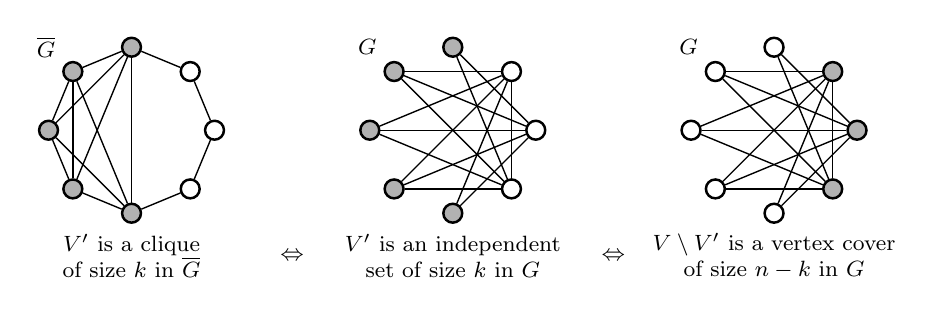
\begin{tikzpicture}[
  scale=0.68,
  font=\footnotesize,
  edge/.style={line width=0.5pt},
  ver/.style={circle,draw=black,line width=0.9pt,minimum size=2.4mm,inner sep=0pt,fill=white},
  sel/.style={ver,fill=gray!60},
]

% ---- parameters ----
\def\h{4}                 % total n = 2h
\pgfmathtruncatemacro{\n}{2*\h}
% \def\k{5}                 % |V'|
\pgfmathtruncatemacro{\k}{\h+1} 
\def\R{1.55}

\pgfmathsetmacro{\step}{360/\n}
% \pgfmathsetmacro{\offset}{270 - \step/2}  % flat bottom edge
\pgfmathsetmacro{\offset}{270}  % peaky bottom node
\pgfmathtruncatemacro{\nminus}{\n-1}
\pgfmathtruncatemacro{\Vstart}{\n-\k+1}   % V' = {Vstart,...,n} (on the left, if k<=h)

% --- place vertices on the circle ---
% mode=0 : highlight V'
% mode=1 : highlight V\V'
\newcommand{\PlaceCycle}[2]{%
  \foreach \i in {1,...,\n}{%
    \pgfmathsetmacro{\ang}{\i*\step+\offset}%
    \edef\mystyle{ver}%
    \ifnum#2=0 % highlight V'
      \ifnum\i<\Vstart\relax\else\edef\mystyle{sel}\fi
    \else      % highlight V\V'
      \ifnum\i<\Vstart\relax\edef\mystyle{sel}\fi
    \fi
    \node[\mystyle] (#1\i) at (\ang:\R) {};%
  }%
}


% ========================= Left: \bar G =========================
\begin{scope}[shift={(0,0)}]
  \PlaceCycle{l}{0}

  %  % debugging: add labels to vertices
  % \foreach \i in {1,...,\n}{%
  %   \node at (\i*360/\n+\offset:\R+0.25) {\i};%
  % }%
  % \node[above, outer sep = 5pt] at (l\Vstart) {$v_{\text{start}}$};

  % edges clique
  \foreach \i in {\Vstart,...,\nminus}{%
    \pgfmathtruncatemacro{\ip}{\i+1}%
    \foreach \j in {\ip,...,\n}{%
      \draw[edge] (l\i)--(l\j);%
    }%
  }%
  % remaining outer circle edges
  \foreach \i in {1,...,\Vstart}{%
    \pgfmathtruncatemacro{\iminus}{\i-1}%
    \ifnum\iminus=0\relax\pgfmathtruncatemacro{\iminus}{\n}\fi
    \draw[edge] (l\iminus)--(l\i);%
  }%

  \node[anchor=west] at (-1.95,1.55) {$\overline{G}$};
  \node[align=center] at (0,-2.35)
    {$V'$ is a clique\\ of size $k$ in $\overline{G}$};
\end{scope}

\node at (3,-2.35) {$\Leftrightarrow$};

% ========================= Middle: G =========================
\begin{scope}[shift={(6,0)}]
  \PlaceCycle{m}{0}
  \pgfmathtruncatemacro{\Vstartm}{\Vstart-1}%
  \foreach \i in {1,...,\Vstartm}{
    \pgfmathtruncatemacro{\ipp}{\i+2}%
    \foreach \j in {\ipp,...,\n}{
      \ifnum\i=1\relax
      \ifnum\j=\n\relax
        % skip edge (1,n)
      \else
        \draw[edge] (m\i)--(m\j);%
      \fi
    \else
      \draw[edge] (m\i)--(m\j);%
    \fi
    }
  }

  \node[anchor=west] at (-1.95,1.55) {$G$};
  \node[align=center] at (0,-2.35)
    {$V'$ is an independent\\set of size $k$ in $G$};
\end{scope}

\node at (9,-2.35) {$\Leftrightarrow$};

% ========================= Right: G (vertex cover highlighted) =========================
\begin{scope}[shift={(12,0)}]
  \PlaceCycle{r}{1}
    \pgfmathtruncatemacro{\Vstartm}{\Vstart-1}%
  \foreach \i in {1,...,\Vstartm}{
    \pgfmathtruncatemacro{\ipp}{\i+2}%
    \foreach \j in {\ipp,...,\n}{
      \ifnum\i=1\relax
      \ifnum\j=\n\relax
        % skip edge (1,n)
      \else
        \draw[edge] (r\i)--(r\j);%
      \fi
    \else
      \draw[edge] (r\i)--(r\j);%
    \fi
    }
  }

  \node[anchor=west] at (-1.95,1.55) {$G$};
  \node[align=center] at (0,-2.35)
    {$V\setminus V'$ is a vertex cover\\ of size $n-k$ in $G$};
\end{scope}

\end{tikzpicture}
\]

\begin{proof}
We prove the implications in the following triangle:
\(
\newcommand{\scalefraction}{0.68}
\begin{tikzcd}[column sep={\scalefraction*1cm,between origins},
               row sep={\scalefraction*1.732050808cm,between origins},
               arrows=Rightarrow]
  & \ref{lem:civc-clique}
    \arrow[dr,""{pos=.5,sloped,overlay, inner sep=0pt,
      label={[black]center:\hyperlink{proof:civc-1-2}{\phantom{\rule{10pt}{15pt}}}}}]
  &
  \\
  \ref{lem:civc-vertex-cover}
    \arrow[ur,""{pos=.5,sloped,overlay, inner sep=0pt,
      label={[black]center:\hyperlink{proof:civc-3-1}{\phantom{\rule{10pt}{15pt}}}}}]
  &
  &
  \ref{lem:civc-independent}
    \arrow[ll,""{pos=.5,sloped,overlay, inner sep=0pt,
      label={[black]center:\hyperlink{proof:civc-2-3}{\phantom{\rule{15pt}{5pt}}}}}]
\end{tikzcd}
\)

\vspace{-2\baselineskip}
\hypertarget{proof:civc-1-2}{
\underline{\ref{lem:civc-clique} $\Rightarrow$ \ref{lem:civc-independent}:}}

If \(V'\) is a clique in \(\overline{G}\),
then for each \(u,v \in V'\), \((u,v)\) is an edge of \(\overline{G}\)
implying that \((u, v)\) is not an edge of \(G\),
implying that \(V'\) is an independent set in \(G\).
\tikzmark{edge_mark}
\definecolor{vertRed}{RGB}{204, 1, 0}
\begin{tikzpicture}[remember picture,overlay, font=\footnotesize,
  myedge/.style={line width=0.5pt},
  myvert/.style={circle,draw=black,line width=0.9pt,minimum size=2.4mm,inner sep=0pt,fill=vertRed},
]
\coordinate (edge) at (pic cs:edge_mark);
\coordinate (left) at ($(edge)+(1.4,-0.22)$);
\node[myvert] (u) at (left) {};
\node[myvert] (v) at ($(left)+(1.2,0)$) {};
% \draw[myedge] (u) -- (v);
\node[anchor=east] at (u.west) {$u$};
\node[anchor=west] at (v.east) {$v$};
\end{tikzpicture}

\hypertarget{proof:civc-2-3}{
\underline{\ref{lem:civc-independent} $\Rightarrow$ \ref{lem:civc-vertex-cover}:}}

\autoref{claim:vc_equiv_is}.

\hypertarget{proof:civc-3-1}{
\underline{\ref{lem:civc-vertex-cover} $\Rightarrow$ \ref{lem:civc-clique}:}}

% If V\V′ is a vertex cover for G, then for any u,v ∈ V′ there is no edge (u,v) in G (because not covered by V\V’), implying that there is an edge (u,v) in G, implying that V ′ is a clique in G.
If \(V \setminus V'\) is a vertex cover for \(G\),
then for any \(u,v \in V'\) there is no edge \((u,v)\) in \(G\) (because not covered by \(V \setminus V'\)),
implying that there is an edge \((u,v)\) in \(\overline{G}\),
implying that \(V'\) is a clique in \(\overline{G}\).

This closes the triangle of implications and proves \autoref{lem:clique_independent_vc}.
\end{proof}




\subsubsection{Dominating Set}\label{sec:dominating_set}

\begin{definition}[Dominating Set]\label{def:dominating-set}
  A dominating set in a graph \(G=(V,E)\) is a subset of vertices \(V' \subseteq V\)
  such that every vertex in the graph is either in \(V'\) or is adjacent to some vertex in \(V'\).
\end{definition}
\begin{problem}[Dominating Set]\label{prob:dominating-set}
Given a graph \(G=(V,E)\) and an integer \(k\),
does \(G\) have a dominating set of size \(k\)?
\end{problem}

\textcolor{AccentBlue}{Dominating Set is NP-complete}.
Reduction from \nameref{prob:vertex-cover}. 
\(\text{\hyperref[prob:vertex-cover]{VC}} \leq_{P} \text{\hyperref[prob:dominating-set]{DS}}\).

\begin{caution}
Note:
\begin{itemize}
\item
If \(G\) has no isolated vertices, a vertex cover for \(G\) is a dominating set for \(G\).
\item
But a dominating set for \(G\) need not be a vertex cover
\qedhere
\end{itemize}
\end{caution}

\textcolor{AccentBlue}{Transformation from \hyperref[prob:vertex-cover]{VC} to \hyperref[prob:dominating-set]{DS}}.
\begin{itemize}
\item
Given \((G,k)\) an instance of \hyperref[prob:vertex-cover]{VC},
produce \((G',k')\) an instance of \hyperref[prob:dominating-set]{DS} such that
\(G\) has a vertex cover of size \(k\) iff \(G'\) has a dominating set of size \(k'\).
\item
Let \(V'\) be the VC of \(G\).
Let \(V''\) be the DS of \(G'\).
\item
\textcolor{AccentBlue}{Observation}.
If \(G\) has isolated vertices we must include them in \(V''\).
\item
Map the notion of ``incident edge'' to notion of ``adjacent vertex''.
Map edges to vertices.
\end{itemize}

So, given \((G,k)\) for \hyperref[prob:vertex-cover]{VC} create graph \(G'\) as follows:
\begin{itemize}
\item
Initially, \(G' = G\).
\item
For each edge \((u,v)\) in \(G\) we create a new vertex \(w_{uv}\) in \(G'\).
\item 
Add edges \((u, w_{uv})\) and \((v, w_{uv})\) in \(G'\).
\item
Let \(I\) denote the set of isolated vertices in \(G\).
\item
Set \(k' = k + |I|\).
\item
Output \((G', k')\).
\end{itemize}




\begin{lemma}\label{lem:vc_reduces_to_ds}
\(G\) has a vertex cover of size \(k\) iff \(G'\) has a dominating set of size \(k'\).
\end{lemma}
\begin{proof}
`\(\Rightarrow\)' (if \(V'\) is a vertex cover for \(G\), then \(V'' = V' \cup I\) is a dominating set for \(G'\)):
Indeed all vertices of \(G'\) are either in \(V''\) or adjacent to \(V''\).
\(|V''| = |V'| + |I| \leq k + |I| = k'\).

`\(\Leftarrow\)' (if \(G'\) has a dominating set \(V''\) of size \(k'\) then \(G\) has a vertex cover of size \(k = k' - n_I\)):
All isolated vertices of \(G'\) must be in \(V''\).
Let \(V'''\) = \(V'' \setminus V_I\) be the remaining \(k = k' - n_I\) vertices.
Modify \(V'''\) so that it contains no middle vertex 
(substitute the ``middle vertex'' by any adjacent regular vertex. Still dominates the same vertices).
Let \(V'\) be the resulting set.
\(V'\) must be a \hyperref[prob:vertex-cover]{VC} of \(G\)
(if an edge not covered then middle vertex not adjacent to DS).
\(V'\) must be a vertex cover for \(G\).
If there is a edge \((u,v)\) in \(G\) not covered by \(V'\) 
(neither \(u\) nor \(v\) is in \(V'\)),
then the middle vertex \(w_{uv}\) would not be adjacent to any vertex of \(V''\) in \(G'\).
This contradicts that \(V''\) was a dominating set for \(G'\).
\end{proof}
























\subsection{NP-Completeness}\label{sec:np_completeness}

\subsubsection{Complexity Classes}
\textcolor{AccentBlue}{Complexity class}:
collection of languages (decision problems), which are similar in terms of how hard it is to determine membership (solve).

Recall \autoref{def:P}:
P is the set of all languages (i.e., decision problems) for which membership can be \emph{determined} in (worst case) polynomial time.

\nameref{def:P} is a complexity class

\renewcommand{\arraystretch}{1.35}
\setlength{\tabcolsep}{0.5pt}
\arrayrulecolor{black}
\begin{tabularx}{\linewidth}{|>{\arraybackslash}p{0.16\linewidth}|>{\arraybackslash}X|>{\arraybackslash}p{0.28\linewidth}|}
\hline
{ Problem}      & { Description}                                          & { Algorithm} \\
\hhline{|=|=|=|}
Multiple        & Is $x$ a multiple of $y$?                               & Grade school division \\
\hline
RelPrime        & Are $x$ and $y$ relatively prime?                       & Euclid (300 BCE) \\
\hline
Primes          & Is $x$ prime?                                           & AKS (2002) \\
\hline
Edit-Distance   & Is the edit distance between $x$ and $y$ less than 5?   & Dynamic programming \\
\hline
LSolve          & Is there a vector $x$ that satisfies $Ax=b$?            & Gauss-Edmonds elim. \\
\hline
\end{tabularx}

Not all languages are in \nameref{def:P}.

\begin{definition}[Simple Cycle]\label{def:simple-cycle}
Given a graph \(G=(V,E)\),
a simple cycle is a closed path that visits each vertex at most once.
\end{definition}

\begin{problem}[Hamiltonian Cycle]\label{prob:ham-cycle}
Given a graph \(G=(V,E)\),
does \(G\) contain a \nameref{def:simple-cycle} that visits each vertex exactly once?
\end{problem}
or in terms of languages:
\[
\text{HC} = \{  G  \mid \text{\(G\) has a simple cycle that visits all vertices}\}
\]

There is no known polynomial time algorithm for \autoref{prob:ham-cycle}.

NP: non-deterministic polynomial time.

alternative (equivalent) definition (to avoid non-determinism):
set of all languages (i.e., decision problems) for which membership can be \emph{verified} in (worst case) polynomial time.


A decision problem (language recognition problem) may be hard to solve, but, given a string \(y\) (a potential solution) it may be easy to verify that \(y\) corresponds to a solution, a yes answer of the decision problem.
\begin{example}[Hamiltonian Cycle Verification]\label{ex:hamiltonian_cycle_verification}
Hard to find a Hamiltonian cycle in a graph.
But suppose that someone gives a permutation of vertices.
then it is easy to check if this is a legal cycle that visits all vertices in the graph exactly once.
So it is easy to \emph{verify} a \nameref{prob:ham-cycle}.

A sequence of vertices that forms a \hyperref[prob:prob:ham-cycle]{HC} is called a \textcolor{AccentRed}{certificate}.
\end{example}


Note that not all decision problems are easy to verify:
\begin{itemize}
\item 
Given a graph \(G\), does \(G\) have a \emph{unique} Hamiltonian cycle?
\[ \text{UHC} = \{ G \mid \text{\(G\) has a unique Hamiltonian cycle} \} \]
\item
Given a graph \(G\), does \(G\) have \emph{no} Hamiltonian cycle?
\[ \overline{\text{HC}} = \{ G \mid \text{\(G\) has no Hamiltonian cycle} \} \]
\end{itemize}
No known polynomial time verification algorithm for either.



\begin{definition}[Certificate]\label{def:certificate}
% Piece of information which allows us to verify that a decision problem has a solution (a Yes answer) in polynomial time.
% \end{definition}
% \begin{definition}[Certificate]\label{def:certificate}
Piece of information (a string \(t\)) which helps to verify that an instance \(x\) of problem \(X\) has a solution, i.e. that \(x \in X\).
\end{definition}

\begin{definition}[Certifier]\label{def:certifier}
An algorithm \(C(s, t)\) is a \emph{certifier} (also called \emph{verification algorithm}), if for every string \(s\) with \(s \in X\) (\(s\) is a yes instance of \(X\)), 
iff there exists a string \(t\) such that \(C(s, t) = \text{Yes}\).
\begin{itemize}
\item
\(s\): input string (a possible instance of problem \(X\))
\item
\(t\): certificate
\item
for a poly-time certifier, \(|t| \leq p(|s|)\) for some polynomial \(p(\cdot)\)
\end{itemize}
Note, \(C(s, t) = \text{No}\) when \(t\) is not a certificate.
\(C\) is a Yes/No algorithm.
\end{definition}

\begin{definition}[NP]\label{def:NP}
decision problems for which there exists a \emph{poly-time} certifier, i.e. 
\(C(s,t)\) is a poly-time algorithm and \(|t| \leq p(|s|)\) for some polynomial \(p(\cdot)\).
\end{definition}


\begin{problem}[Composites]\label{prob:composites}
Given an integer \(s\), is \(s\) composite (i.e., not prime)?
\end{problem}

\textcolor{AccentBlue}{Certificate}. 
A non-trivial factor \(t\) of \(s\) (i.e., \(1 < t < s\) and \(t \mid s\)).
Note that such a certificate exists iff \(s\) is composite.
Moreover \(|t| \leq |s|\).

\begin{algorithm}[h]
\caption{Certifier for \nameref{prob:composites}}
\label{alg:certifier-composites}
\begin{algorithmic}[1]
\Function{BooleanC}{$s, t$}
  \If{$t \leq 1 \OR t \geq s$} \Return false
  \ElsIf{$s$ is a multiple of $t$} \Return true
  \Else \ \Return false
  \EndIf
\EndFunction
\end{algorithmic}
\end{algorithm}

\textcolor{AccentBlue}{Conclusion}.
\nameref{prob:composites} is in NP.


\begin{fact}\label{fact:sat_in_np}
For \nameref{prob:sat} a \textcolor{AccentBlue}{\nameref{def:certificate}} is a satisfying assignment of variables
and the \textcolor{AccentBlue}{\nameref{def:certifier}} checks that each clause in \(\Phi\) has at least one true ltieral.
\end{fact}

\textcolor{AccentBlue}{Conclusion}.
\nameref{prob:sat} is in NP.

\begin{fact}\label{fact:ham_cycle_in_np}
For \hyperref[prob:ham-cycle]{HC} a \textcolor{AccentBlue}{\nameref{def:certificate}} is a permutation of the \(n\) nodes (which is a Ham. cycle if \(G\) has one)
and the \textcolor{AccentBlue}{\nameref{def:certifier}} checks that the certificate contains each node in \(V\) exactly once and that there is an edge between each pair of adjacent nodes in the permutation.
\end{fact}

\textcolor{AccentBlue}{Conclusion}.
\nameref{prob:ham-cycle} is in NP.

\medskip

\textcolor{AccentBlue}{P}: Decision problems for which there is a \textcolor{AccentRed}{poly-time algorithm}.

\textcolor{AccentBlue}{NP}: Decision problems for which there is a \textcolor{AccentRed}{poly-time certifier}.

\textcolor{AccentBlue}{EXP}: Decision problems for which there is a \textcolor{AccentRed}{exponential-time algorithm}.


\begin{claim}
\(\text{P} \subseteq \text{NP}\).
\end{claim}
\begin{proof}
Consider any problem \(X\) in P.
There exists a poly-time algorithm \(A(s)\) that solves \(X\): 
returns yes, if \(s \in X\), and returns no, otherwise.
Then there exists a poly-time certifier.
Certificate: \(t = \epsilon\) (empty string),
certifier \(C(s, t) = A(s)\).
Thus, \(X\) in NP.
\end{proof}



\begin{claim}
\(\text{NP} \subseteq \text{EXP}\).
\end{claim}
\begin{proof}
Consider any problem \(X\) in NP.
Since \(X\) is in NP, there exists a polynomial time certifier \(C(s, t)\) for \(X\).
Let \(p(|s|)\) be the polynomial time complexity of \(C(s,t)\); \(|t| \leq p(|s|)\).

We construct an algorithm that solves \(X\) on instance \(s\), based on \(C(s, t)\) (use brute force):
\begin{itemize}
\item
Generate all strings \(t\) with \(|t| \leq p(|s|)\).
Run \(C(s, t)\) on each string \(t\).
\item
If \(C(s, t)\) returns \texttt{yes} for any such string \(t\), stop and return \texttt{yes}.
\item
There is an exponential number of possible such strings \(t\), given \(p(|s|)\).
Thus, this is an exponential-time algorithm.
\item
After \(\leq p(|s|)\) rounds the algorithm stops with a \texttt{yes} or \texttt{no} answer.
\qedhere
\end{itemize}
\end{proof}


\begin{openquestion}[P vs NP]
Is $\mathrm{P}=\mathrm{NP}$, i.e. is the decision problem as easy as the verification problem?
\end{openquestion}
The consesus is probably no. There is \$1M prize for proof.




% \begin{tikzpicture}[x=1cm,y=1cm,>=Stealth]

% % --- parameters (keep consistent) ---
% \def\xL{3.0}   \def\yC{4.35} \def\rNP{2.10}
% \def\xR{9.0}
% \def\yRef{2.20}

% % --- horizontal dotted reference line ---
% \draw[gray!65, dotted, line width=0.8pt] (0,\yRef) -- (12,\yRef);

% % --- center complexity axis ---
% \draw[line width=1pt,->] (6,0) -- (6,8);
% \node[rotate=90] at (5.72,3.95) {Complexity};

% % ===================== LEFT: P != NP =====================

% % NP (circle)
% \draw[line width=0.1pt] (\xL,\yC) circle[radius=\rNP];

% % P : shares a SHORT ARC with NP (coincide, then diverge)

% \begin{scope}
%   \path (\xL,\yC) coordinate (cL);

%   \def\angL{250}
%   \def\angR{290}

%   % points on the NP boundary circle
%   \coordinate (pL) at ($(cL)+(\angL:\rNP)$);
%   \coordinate (pR) at ($(cL)+(\angR:\rNP)$);

%   % apex (topmost point of the dotted region)
%   \def\h{-0.5}
%   \coordinate (pA) at ($(cL)+(0,\h)$);

%   % tangent-handle lengths (tune these)
%   \def\t{0.6}  % handles at circle junctions
%   \def\a{1.2}  % handles at apex (horizontal)

%   % unit-ish tangent directions at circle points (CCW tangent)
%   \path let \p1 = ($(pL)-(cL)$) in coordinate (tL) at (-\y1,\x1);
%   \path let \p2 = ($(pR)-(cL)$) in coordinate (tR) at (-\y2,\x2);

%   % C1 at apex: last control of first spline and first control of second spline
%   % lie on the horizontal tangent through pA, mirrored.
%   \coordinate (cAin)  at ($(pA)+(\a,0)$);   % for segment ending at pA
%   \coordinate (cAout) at ($(pA)+(-\a,0)$);  % for segment starting at pA

%   \draw[densely dotted, thick]
%     (pL)
%       arc[start angle=\angL, end angle=\angR, radius=\rNP]
%     (pR)
%       .. controls ($(pR)+\t*(tR)$) and (cAin)  .. (pA)
%       .. controls (cAout) and ($(pL)-\t*(tL)$) .. (pL);
% \end{scope}


% % ---------- NP-hard (left) : Bezier -> circle arc -> Bezier ----------
% \begin{scope}
%   % endpoints at the top border of the left panel
%   \coordinate (S) at (0.5,8);
%   \coordinate (E) at (5.5,8);

%   % middle arc circle (TUNE THESE THREE)
%   \coordinate (C) at (3.00,6.6); % center of the NP-hard middle arc
%   \def\ain{250}                   % angle where we ENTER the arc
%   \def\aout{290}                  % angle where we LEAVE the arc

%   % join points on the circle
%   \coordinate (Jin)  at ($(C)+(\ain:\rNP)$);
%   \coordinate (Jout) at ($(C)+(\aout:\rNP)$);

%   % tangents at join points (CCW tangent = rotate radius by +90°)
%   \path let \p1 = ($(Jin)-(C)$)  in coordinate (Tin)  at (-\y1,\x1);
%   \path let \p2 = ($(Jout)-(C)$) in coordinate (Tout) at (-\y2,\x2);

%   % handle length along tangent (TUNE)
%   \def\k{0.8}

%   % also steer the ends downward a bit (TUNE these if needed)
%   \coordinate (cS) at ($0.5*($(Jin)-\k*(Tin)$)+0.5*(S)$);
%   \coordinate (cE) at ($0.5*($(Jout)+\k*(Tout)$)+0.5*(E)$);

%   \draw[gray, line width=0.9pt]
%     (S)
%       .. controls (cS) and ($(Jin)-\k*(Tin)$) .. (Jin)
%       arc[start angle=\ain, end angle=\aout, radius=\rNP]
%     (Jout)
%       .. controls ($(Jout)+\k*(Tout)$) and (cE) .. (E);
% \end{scope}

% % labels
% \node at (\xL,6.95) {NP-Hard};
% \node at (\xL,5.45) {NP-Complete};
% \node at (\xL-1.2,4.35) {NP};
% \node at (\xL,3.0) {P};
% \node[font=\Large] at (\xL,1.15) {$\mathrm{P}\ \ne\ \mathrm{NP}$};


% % ===================== RIGHT: P = NP =====================

% % big circle (P = NP = NP-Complete)
% \draw[line width=1pt] (\xR,\yC) circle[radius=\rNP];

% \node at (\xR,6.95) {NP-Hard};
% \node[align=center] at (\xR,5.05) {P $=$ NP $=$\\ NP-Complete};
% \node[font=\Large] at (\xR,1.15) {$\mathrm{P}\ =\ \mathrm{NP}$};



% \begin{scope}
%    % endpoints at the top border of the left panel
%   \coordinate (S) at (6.5,8);
%   \coordinate (E) at (11.5,8);

%   % middle arc circle (TUNE THESE THREE)
%   \coordinate (C) at (9.00,4.34); % center of the NP-hard middle arc
%   \def\ain{210}                   % angle where we ENTER the arc
%   \def\aout{330}                  % angle where we LEAVE the arc

%   % join points on the circle
%   \coordinate (Jin)  at ($(C)+(\ain:\rNP)$);
%   \coordinate (Jout) at ($(C)+(\aout:\rNP)$);

%   % tangents at join points (CCW tangent = rotate radius by +90°)
%   \path let \p1 = ($(Jin)-(C)$)  in coordinate (Tin)  at (-\y1,\x1);
%   \path let \p2 = ($(Jout)-(C)$) in coordinate (Tout) at (-\y2,\x2);

%   % handle length along tangent (TUNE)
%   \def\k{0.6}

%   % also steer the ends downward a bit (TUNE these if needed)
%   \coordinate (cS) at ($0.5*($(Jin)-\k*(Tin)$)+0.5*(S)$);
%   \coordinate (cE) at ($0.5*($(Jout)+\k*(Tout)$)+0.5*(E)$);

%   \draw[gray, line width=0.9pt]
%     (S)
%       .. controls (cS) and ($(Jin)-\k*(Tin)$) .. (Jin)
%       arc[start angle=\ain, end angle=\aout, radius=\rNP]
%     (Jout)
%       .. controls ($(Jout)+\k*(Tout)$) and (cE) .. (E);
% \end{scope}



% \end{tikzpicture}









If yes: efficient algorithms for \hyperref[prob:3-color]{3-COLOR}, \hyperref[prob:tsp]{TSP}, \hyperref[prob:factor]{FACTORING}\tikzmark{fact_mark}, \hyperref[prob:sat]{SAT}, ...
\definecolor{vertRed}{RGB}{204, 1, 0}
\begin{tikzpicture}[remember picture,overlay, font=\footnotesize]
\coordinate (fact) at (pic cs:fact_mark);
\coordinate (tiploc) at ($(fact)+(-0.1,0.3)$);
\draw[<-] (tiploc) -- ++(0.6,0.45) node[anchor=south west, outer sep = 0pt, inner sep = 0pt] {would break RSA};
\end{tikzpicture}

If no: no efficient algorithms for \hyperref[prob:3-color]{3-COLOR}, \hyperref[prob:tsp]{TSP}, \hyperref[prob:factor]{FACTORING}, \hyperref[prob:sat]{SAT}, ...

\[
% needs: \usetikzlibrary{calc}
\begin{tikzpicture}[scale=0.75,>=Stealth, font=\footnotesize]

% ---- params ----
\def\xL{3}\def\xR{9}\def\yC{4.35}\def\r{2.10}\def\yRef{2.20}

% ---- helpers (compact) ----
\tikzset{pDots/.style={densely dotted,thick},hard/.style={gray,line width=.9pt}}
\newcommand{\tangent}[3]{% #1=(out coord name) #2=center #3=point
  \path let \p1=($(#3)-(#2)$) in coordinate (#1) at (-\y1,\x1);
}
\newcommand{\Pregion}[5]{% center, r, angL, angR, apex-y-offset
  \begin{scope}
    \coordinate (c) at (#1);
    \def\angL{#3}\def\angR{#4}
    \coordinate (L) at ($(c)+(\angL:#2)$);
    \coordinate (R) at ($(c)+(\angR:#2)$);
    \coordinate (A) at ($(c)+(0,#5)$);
    \def\t{0.6}\def\a{1.2} % tweak if you want
    \tangent{tL}{c}{L}\tangent{tR}{c}{R}
    \draw[pDots]
      (L) arc[start angle=\angL,end angle=\angR,radius=#2]
      (R) .. controls ($(R)+\t*(tR)$) and ($(A)+(\a,0)$) .. (A)
          .. controls ($(A)+(-\a,0)$) and ($(L)-\t*(tL)$) .. (L);
  \end{scope}
}
\newcommand{\NPhard}[6]{% S, E, C, r, ain, aout  (k fixed inside; change if needed)
  \begin{scope}
    \coordinate (S) at (#1);\coordinate (E) at (#2);\coordinate (C) at (#3);
    \def\ain{#5}\def\aout{#6}\def\k{#4} % use #4 as "k" (handle length), radius is global \r
    \coordinate (I) at ($(C)+(\ain:\r)$);
    \coordinate (O) at ($(C)+(\aout:\r)$);
    \tangent{tI}{C}{I}\tangent{tO}{C}{O}
    \coordinate (cS) at ($.5*(S)+.5*($(I)-\k*(tI)$)$);
    \coordinate (cE) at ($.5*(E)+.5*($(O)+\k*(tO)$)$);
    \draw[hard]
      (S) .. controls (cS) and ($(I)-\k*(tI)$) .. (I)
      arc[start angle=\ain,end angle=\aout,radius=\r]
      (O) .. controls ($(O)+\k*(tO)$) and (cE) .. (E);
  \end{scope}
}

% ---- background stuff ----
\draw[gray!65,dotted,line width=.8pt] (0,\yRef) -- (12,\yRef);
\draw[line width=1pt,->] (6,1) -- (6,8);
\node[rotate=90] at (5.72,3.95) {Complexity};

% ---- left: P != NP ----
\draw[line width=1pt] (\xL,\yC) circle[radius=\r];
\Pregion{\xL,\yC}{\r}{250}{290}{-0.5}
\NPhard{0.5,8}{5.5,8}{3.0,6.6}{0.8}{250}{290}

\node at (\xL,7.25) {NP-Hard};
\node at (\xL,5.45) {NP-Complete};
\node at (\xL-1.25,4.2) {NP};
\node at (\xL,3.0) {P};
\node[] at (\xL,1.5) {$\text{P} \ne \text{NP}$};

% ---- right: P = NP ----
\draw[line width=1pt] (\xR,\yC) circle[radius=\r];
\NPhard{6.5,8}{11.5,8}{9.0,4.34}{0.6}{210}{330}

\node at (\xR,7.25) {NP-Hard};
\node[align=center] at (\xR,4.5) {P $=$ NP $=$\\ NP-Complete};
\node[] at (\xR,1.5) {$\text{P} = \text{NP}$};

\end{tikzpicture}
\]


\begin{definition}[NP-Hard]\label{def:np-hard}
A problem \(Y\) with the property that for every problem \(X\) in NP, \(X \leq_{P} Y\).
\end{definition}
\begin{definition}[NP-Complete]\label{def:np-complete}
A problem \(Y\) that is in NP and is NP-hard.
\end{definition}

\hl{If one NP-complete problem is found to have a poly time algorithm, then all problems in NP have}

\begin{theorem}
  Suppose \(Y\) is an NP-complete problem.
  \(Y\) is solvable in polynomial time iff P = NP.
\end{theorem}
\begin{proof}
`\(\Leftarrow\)' (if):
If P = NP, then \(Y\) can be solved in poly-time since \(Y\) is in P.

`\(\Rightarrow\)' (only if):
Suppose \(Y\) can be solved in poly-time.
Let \(X\) be any problem in NP.
Since \(X \leq_{P} Y\) and \(Y\) can be solved in poly-time,
we can solve \(X\) in poly-time.
Thus, \(X\) in P, \(\text{NP} \subseteq \text{P}\).
We already know \(\text{P} \subseteq \text{NP}\).
Thus, P = NP.
\end{proof}

\subsubsection{NP-complete Problems}
\begin{fundamentalquestion*}
Do there exist ``natural'' NP-complete problems?
\end{fundamentalquestion*}

\begin{problem}[CIRCUIT-SAT]\label{prob:circuit-sat}
Given a combinational logic circuit built out of AND, OR, and NOT gates,
is there a way to set the input so that the output is 1?
\end{problem}

\begin{theorem}[Cook 1971, Levin 1973]\label{thm:circuit-sat-np-complete}
\hyperref[prob:circuit-sat]{CIRCUIT-SAT} is NP-complete.
\end{theorem}
\begin{proof}[sketch]
Membership in NP is immediate, so we focus on NP-hardness:
 \begin{itemize}
  \item Any algorithm that takes a fixed number of bits $n$ as input and
  produces a yes/no answer can be represented by a circuit.
  Further, if algorithm takes poly in $n$ time, then circuit has poly-size.
    \begin{itemize}
    \item
    sketchy part of proof: fixing the number of bits is important,
    and reflects basic distinction between algorithms and circuits
    \end{itemize}
  \item Consider some problem $X$ in NP. It has a poly-time certifier $C(s,t)$.
  To determine whether $s$ is in $X$, need to know if there exists a
  certificate $t$ of length $\le p(|s|)$ such that $C(s,t)=\texttt{yes}$.

  \item $C(s,t)$ is an algorithm on $|s|+p(|s|)$ bits (input $s$, certificate $t$).
  For fixed input length $|s|$, $C(\cdot,\cdot)$ is an algorithm of fixed input length,
  so we convert it into a poly-size circuit family such that $K_s$ is satisfiable iff
  $C(s,t)=\texttt{yes}$ for some $t$.
  \begin{itemize}
    \item First $|s|$ bits are hard-coded with $s$; remaining $p(|s|)$ bits represent $t$.
  \end{itemize}

  \item $X \le_p \text{\nameref{prob:circuit-sat}}$:
  Given an arbitrary instance $s$ of $X$, transform $s$ (as sketched above) into a poly-size circuit $K_s$
  (in poly time), which is satisfiable iff $s$ is yes instance of $X$.
  \qedhere
 \end{itemize}
\end{proof}

\begin{remark}
  Once we establish first ``natural'' NP-complete problem (\nameref{prob:sat}), others fall like dominoes.
\end{remark}

% \textcolor{AccentBlue}{Recipe to establish NP-completeness of a problem \(Y\)}:
\hl[2]{Recipe to establish NP-completeness of a problem \(Y\)}:
\begin{enumerate}
\item Show that \(Y\) is in NP
\item Choose an NP-complete problem \(X\)
\item Make a reduction: prove that \(X \leq_{P} Y\)
\end{enumerate}

\begin{claim}
  If $X$ is an NP-complete problem and $X \le_p Y$, then $Y$ is NP-hard.
  Further, if $Y$ is in NP, then $Y$ is NP-complete.
\end{claim}
\begin{proof}
Let $W$ be any problem in NP.
Then $W \le_p X \le_p Y$.
By transitivity, $W \le_p Y$.
Thus, $Y$ is NP-hard.
\end{proof}

\begin{theorem}\label{thm:3sat-np-complete}
  \nameref{prob:3-sat} is NP-complete.
\end{theorem}
\begin{proof}
  It suffices to show that \nameref{prob:circuit-sat} $\le_p$ \nameref{prob:3-sat}, since \nameref{prob:3-sat} is in NP.
  Let \(K\) be any circuit.
  Create a 3-CNF formula \(K'\) which is satisfiable iff \(K\) is satisfiable.
  There is a mechanical way to do it (skipped).
\end{proof}




All problems below are NP-complete and polynomially reduce to one another:
\[
\begin{tikzpicture}[
  scale=1.5,
  font=\footnotesize,
  >=Latex,
  group/.style={green!70!black},
  problem/.style={
    draw, fill=gray!10, line width=0.4pt,
    minimum height=5mm, minimum width=22mm,
    inner sep=0pt, align=center,
    font=\footnotesize
  },
  arr/.style={-Latex, line width=0.5pt, outer sep=1pt, inner sep=0pt},
  bluefat/.style={draw=blue!70!black, line width=1.2pt, line join=round},
  bluar/.style={-Latex, draw=blue!70!black, line width=1.2pt, line join=round}
]

% clickable label helper
\newcommand{\plink}[2]{\hyperref[prob:#1]{#2}}
% clickable reduction-label helper (no nested link)
\newcommand{\rref}[1]{\hyperref[#1]{\tiny\autoref*{#1}}}

% --- nodes ---
\node[problem, minimum width=34mm, fill=gray!30] at (0,4.5) (csat) {\plink{circuit-sat}{CIRCUIT-SAT}};
\node[problem, minimum width=20mm] at (0,3.5) (sat3) {\plink{3-sat}{3-SAT}};
\node[group] at (1.5, 4) {Constraint Satisfaction};

\node[problem] at (-3, 3) (cliq) {\plink{clique}{CLIQUE}};
\node[problem] at (-3, 2)(is) {\plink{independent-set}{INDEP. SET}};
\node[problem] at (-3, 1) (vc) {\plink{vertex-cover}{VERTEX COV}};

\node[problem, font=\tiny, minimum height=2.0mm, minimum width=10mm, inner sep=1pt] at (-3.5, 0.35) (domset) {\plink{dominating-set}{DOM. SET}};

\node[problem] at (-3, 0) (sc) {\plink{set-cover}{SET COV}};

\node[group] at (-3, -0.65) {Packing and Covering};

\node[problem] at (-1, 2) (dhc) {\plink{dir-ham-cycle}{DIR-HAM-CYC}};
\node[problem] at (-1, 1) (hc) {\plink{ham-cycle}{HAM-CYC}};
\node[problem] at (-1, 0) (tsp) {\plink{tsp}{TSP}};
\node[group] at (-1, -0.65) {Sequencing};

\node[problem] at (1, 2) (g3c) {\plink{graph-3-color}{GRAPH 3-COL}};
\node[problem] at (1, 1) (ccov) {\plink{clique-cover}{CLIQUE COV}};
\node[group] at (1, -0.65) {Partitioning};

\node[problem] at (3, 2) (ss) {\plink{subset-sum}{SUBSET-SUM}};
\node[problem] at (3, 1) (sch) {\plink{scheduling}{SCHEDULING}};
\node[group] at (3, -0.65) {Numerical};

% % --- black reduction arrows ---

\draw[arr] (csat) -- node[midway, left] {\rref{thm:3sat-np-complete}} (sat3);

\draw[arr] (sat3.south) -- node[pos=0.7, right, anchor=north west, inner sep=1pt, outer sep=0pt] {\rref{claim:3-sat-reduces-to-dir-ham-cycle}} (dhc.north);
\draw[arr] (sat3.south) -- (g3c.north);
% \draw[arr] (sat3.south) -- node[midway, right] {\rref{thm:3sat-to-3color}} (g3c.north);
\draw[arr] (sat3.south) -- (ss.north);
% \draw[arr] (sat3.south) -- node[midway, right] {\rref{thm:3sat-to-subset-sum}} (ss.north);

\def\myshift{0.1}

\draw[arr] (sat3.south) -- node[pos=0.7, right, anchor=north west, inner sep=1pt, outer sep=0pt] {\rref{claim:3sat_reduces_to_is}} ($(is.north)!\myshift!(is.north east)$);

\draw[arr, <->] ($(cliq.south)!\myshift!(cliq.south west)$) -- node[midway, left] {\rref{claim:clique_equiv_is_equiv_vc}} ($(is.north)!\myshift!(is.north west)$);

\draw[arr, <->] ($(is.south)!\myshift!(is.south west)$) -- node[midway, left] {\rref{claim:clique_equiv_is_equiv_vc}} ($(vc.north)!\myshift!(vc.north west)$);
\draw[arr] ($(is.south)!\myshift!(is.south east)$) -- node[midway, right] {\rref{claim:vc_equiv_is}} ($(vc.north)!\myshift!(vc.north east)$);


% orange equivalence box (behind CLIQUE / IS / VC) 
\begin{scope}[on background layer]
  \node[
    draw=orange!80!black,
    fill=orange!12,
    rounded corners=2pt,
    line width=0.8pt,
    inner sep=4.5pt,
    fit=(cliq)(is)(vc)
  ] (eqbox) {};
\end{scope}
\node[
  anchor=south west,
  text=orange!80!black,
  font=\scriptsize
] at (eqbox.north west) {equivalent (\rref{lem:clique_independent_vc})};


\draw[arr] (vc) -- node[midway, right] {\rref{claim:vc_reduces_to_sc}} (sc);
\draw[arr] (vc) -- node[pos=0.5, left, inner sep=1pt] {\rref{lem:vc_reduces_to_ds}} (domset);


% \draw[arr] (dhc) -- (hc);
\draw[arr] (dhc) -- node[midway, right] {\rref{claim:dir-ham-cycle-reduces-to-ham-cycle}} (hc);
% \draw[arr] (hc) -- (tsp);
\draw[arr] (hc)  -- node[midway, right] {\rref{claim:ham-cycle-reduces-to-tsp}} (tsp);

\draw[arr] (g3c) -- node[midway, right] {\rref{claim:3col_reduces_to_clique_cover}} (ccov);
\draw[arr] (ss) -- (sch);
% \draw[arr] (ss)  -- node[midway, right] {\rref{thm:subset-sum-to-scheduling}} (sch);


% % labeled arrow to INDEPENDENT SET
% \draw[arr] (sat3) -- node[midway, above, sloped, align=left]
%   {3-SAT reduces to\\INDEPENDENT SET} (is);

% --- blue arrows ---
\coordinate (BL) at (-4.2, 0);
\coordinate (BR) at (4.2, 0);
\coordinate (TR) at ($(csat) + (4.2, 0)$);
\coordinate (TL) at ($(csat) + (-4.2, 0)$);
\draw[bluar] (tsp) -- (BR) -- (TR) -- node[pos=0.45, above] {\tiny by definition of NP-completeness} (csat);
\draw[bluefat] (ccov.south) -- ($(ccov.south |- BL)$);
\draw[bluefat] (sch.south) -- ($(sch.south |- BL)$);
\draw[bluar] (sc) -- (BL) -- (TL) -- node[pos=0.45, above] {\tiny \autoref{thm:circuit-sat-np-complete}} (csat);
\draw[bluefat] (domset.west) -- ($(domset.west -| BL)$);

\end{tikzpicture}
\]


Basic categories of NP-complete problems and paradigmatic examples:
\begin{itemize}
  \item Packing problems: \hyperref[prob:set-packing]{SET PACKING}, \hyperref[prob:independent-set]{INDEPENDENT SET}
  \item Covering problems: \hyperref[prob:set-cover]{SET COVER}, \hyperref[prob:vertex-cover]{VERTEX COVER}
  \item Constraint satisfaction problems: \hyperref[prob:sat]{SAT}, \hyperref[prob:3-sat]{3-SAT}
  \item Sequencing problems: \hyperref[prob:ham-cycle]{HAM-CYCLE}, \hyperref[prob:tsp]{TSP}
  \item Partitioning problems: \hyperref[prob:3d-matching]{3D-MATCHING}, \hyperref[prob:graph-3-color]{3-COLOR}
  \item Numerical problems: \hyperref[prob:subset-sum]{SUBSET-SUM}, \hyperref[prob:knapsack]{KNAPSACK}
\end{itemize}

In practice, most problems are either known to be in P or known to be NP-complete.
Notable exeptions: Factoring, graph isomorphism, Nash equilibrium.


\begin{problem}[3Col]\label{prob:graph-3-color}
Given a graph \(G\), can each of its vertices be labeled with one of three different ``colors'' such that no two adjacent vertices have the same label?
\begin{itemize}
\item arises in various partitioning problems (adjacent object not in same group)
\item planar graphs can be colored with 4 colors (well known)
\item determining if 3 colors are possible is hard (even for planar graphs)
\item \nameref{prob:graph-3-color} is known to be NP-complete
\qedhere
\end{itemize}
\end{problem}

\begin{problem}[Clique Cover]\label{prob:clique-cover}
Given a graph \(G=(V,E)\) and an integer \(k\), can we partition the vertex set into \(k\) cliques?
\begin{itemize}
\item every vertex needs to be in exactly one clique!
\item \autoref{prob:clique-cover} arises in clustering.
\item \(\text{\hyperref[prob:graph-3-color]{3Col}} \leq_{P} \text{\hyperref[prob:clique-cover]{CCov}}\) 
\qedhere
\end{itemize}
\end{problem}

\begin{claim}\label{claim:3col_reduces_to_clique_cover}
  A graph \(G = (V,E)\) is 3-colorable iff its complement \(\overline{G} = (V, \overline{E})\) has a clique cover with \(k=3\) cliques.
\end{claim}

\begin{proof}
`\(\Rightarrow\)': 
Suppose \(G\) is 3-colorable.
Let \(V_1, V_2, V_3\) be the 3 color classes.
Every pair of distinct vertices in \(V_i\) are not adjacent in \(G\).
Thus, they are adjacent in \(\overline{G}\).
So, \(V_i\) forms a complete subgraph in \(\overline{G}\).
Thus, this is a clique cover of size 3 for \(\overline{G}\).

`\(\Leftarrow\)':
Suppose \(\overline{G}\) has a clique cover of size 3, denoted \(V_1, V_2, V_3\).
Give the vertices of \(V_i\) color \(i\), \(i=1,2,3\).
No two vertices in \(V_i\) are adjacent in \(G\).
Thus, this is a legal coloring for \(G\).
\end{proof}


\subsubsection{co-NP and the Asymmetry of NP}\label{sec:co-np}
\textcolor{AccentBlue}{Asymmetry of NP}:
We only have short proofs of \texttt{yes} instances.
We do not necessarily have proofs for \texttt{no} inst  ances.

\begin{example}[SAT vs TAUTOLOGY]\label{ex:sat_vs_tautology}
Can prove a \hyperref[def:CNF]{CNF} formula is satisfiable by giving a truth assignment (\autoref{fact:sat_in_np}).
How could we prove that a formula is \emph{not} satisfiable, i.e., a contradiction?
How can we prove that a formula is always true, i.e., a tautology?
% TAUTOLOGY not known to be in NP.
\end{example}

\begin{example}[HAM-CYCLE vs NO-HAM-CYCLE]\label{ex:ham_cycle_vs_no_ham_cycle}
Can prove that a graph is Hamiltonian by giving a Hamiltonian cycle (\autoref{fact:ham_cycle_in_np}).
How can we prove that a graph is \emph{not} Hamiltonian?
\end{example}


The complement of SAT, i.e. \(\overline{\text{SAT}}\), is the set of all Boolean \hyperref[def:CNF]{CNF} formulas that are not satisfiable,
i.e.,
the CONTRADICTION (formulas that are always false).

\(\text{TAUTOLOGY} \equiv_{P} \text{CONTRADICTION}\): \(\Phi\) is a tautology iff \(\neg \Phi\) is a contradiction.

Thus, \(\overline{\text{SAT}} \equiv \text{CONTRADICTION} \equiv_{P} \text{TAUTOLOGY}\).


\begin{definition}[Complement]\label{def:complement}
Given a decision problem \(X\), its \textcolor{AccentRed}{complement} \(\overline{X}\) is the same problem with the \texttt{yes} and \texttt{no} answers reversed,
i.e.,
\(s\) in \(X\) iff \(s\) not in \(\overline{X}\).
\end{definition}

\begin{definition}[co-NP]\label{def:co-NP}
The \nameref{def:complement}s of decision problems in \nameref{def:NP},
i.e.,
a problem \(X\) belongs to co-NP iff \(\overline{X}\) belongs to NP.
\end{definition}

\setlength{\tabcolsep}{4.5pt}
\begin{tabular}{>{\raggedright\arraybackslash}p{0.25\linewidth} |>{\raggedright\arraybackslash}p{0.25\linewidth}}
{\textcolor{AccentBlue}{Examples \nameref{def:NP}}} & {\textcolor{AccentBlue}{Examples \nameref{def:co-NP}}} \\
\hline
\footnotesize SAT         & \footnotesize TAUTOLOGY \\
\footnotesize HAM-CYCLE   & \footnotesize NO-HAM-CYCLE \\
\footnotesize COMPOSITES  & \footnotesize PRIMES \\
\end{tabular}







\begin{openquestion}
Does $\mathrm{NP}=\mathrm{co\text{-}NP}$?
\begin{itemize}
  \item 
  Do \texttt{yes} instances have succinct certificates iff \texttt{no} instances do?
  \item
  Consensus opinion: no.
  \item
  Easy to get a simple short certificate for most problems in NP but to get a no certificate is often not easy.
  \qedhere
\end{itemize}
\end{openquestion}


\[
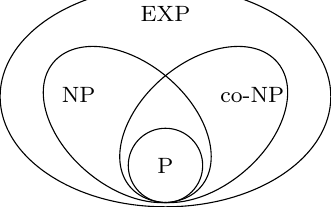
\begin{tikzpicture}[scale=0.35]
  \useasboundingbox (-5,-2.5) rectangle (5,3);

  \draw[rotate around={-40:(-2,0)}] (-1.2,0) ellipse (3.5 and 2.25);
  \draw[rotate around={40:( 2,0)}] ( 1.2,0) ellipse (3.5 and 2.25);
  \node[font=\footnotesize] at (-3.15,0.55) {NP};
  \node[font=\footnotesize] at ( 3.15,0.55) {co-NP};

  \draw (0,-2) circle [radius=1.35];
  \node[font=\footnotesize] at (0,-2) {P};
  
  \draw (0,0.5) ellipse (6 and 4);
  \node[font=\footnotesize] at (0,3.5) {EXP};
\end{tikzpicture}
\]

\begin{claim}\label{claim:p_eq_coP}
\(\mathrm{P} = \mathrm{co\text{-}P}\). 
\end{claim}
\begin{proof}
% If \(X\) is in P, then we can decide \(\overline{X}\) in poly-time by reversing the answer.
If we have an algorithm \(A\) that decides \(X\) in poly-time,
we can design an algorithm \(\overline{A}\) that decides \(\overline{X}\) in poly-time:
Run \(A\) on input \(x\) and flip its answer.
\end{proof}


\begin{theorem}
 If \(\mathrm{NP} \neq \mathrm{co\text{-}NP}\), then \(\mathrm{P} \neq \mathrm{NP}\). 
%  (Contrapositive: If \(\mathrm{P} = \mathrm{NP}\), then \(\mathrm{NP} = \mathrm{co\text{-}NP}\).)
\end{theorem}
\begin{proof}[idea]
% \begin{itemize}
  % \item 
  P is closed under complement (\autoref{claim:p_eq_coP}).
  % \item 
  If P = NP, then NP is also closed under complement, i.e., NP = co-NP.
  % \item 
  Contrapositive yields the result.
%   \qedhere
% \end{itemize}  
\end{proof}


\textcolor{AccentBlue}{Good characterization}. \textcolor{gray!70!black}{[Edmonds 1965]}
\(\text{NP} \cap \text{co-NP}\).
\begin{itemize}
  \item If problem \(X\) is in both NP and co-NP, then:
  \begin{itemize}
    \item for \texttt{yes} instance, there is a succinct certificate
    \item for \texttt{no} instance, there is a succinct disqualifier (certificate)
  \end{itemize}
  \item Provides conceptual leverage for reasoning about a problem.
\end{itemize}

\begin{example}
Given a bipartite graph, is there a perfect matching?
\begin{itemize}
  \item if yes, can exhibit a perfect matching.
  \item if no, can exhibit a set of nodes \(S\) such that \(|N(S)| < |S|\) (\autoref{thm:hall-marriage}).
  \item Bipartite perfect matching is in \(\text{NP} \cap \text{co-NP}\).
  \qedhere
\end{itemize}
\end{example}

\begin{observation}
  \(\text{P} \subseteq \text{NP} \cap \text{co-NP}\).
\end{observation}

\begin{openquestion}
  Does \(\text{P} = \text{NP} \cap \text{co-NP}\)?
  \begin{itemize}
    \item mixed opinions.
    \item many examples where problem found to have non-trivial good characterization, but only years later discovered to be in P.
    \begin{itemize}
      \item linear programming \textcolor{gray!70!black}{[Khachiyan, 1979]}
      \item primality testing \textcolor{gray!70!black}{[Agrawal-Kayal-Saxena, 2002]}
      \qedhere
    \end{itemize}
  \end{itemize}
\end{openquestion}

\begin{fact}
  Factoring is in \(\text{NP} \cap \text{co-NP}\), but not known to be in P.%
  \footnote{if poly-time algorithm for factoring, can break RSA cryptosystem.}
\end{fact}




\subsubsection{Sequencing Problems}\label{sec:sequencing_problems}

\begin{example}%[Hamiltonian Cycle]
Vertices and faces of a dodecahedron have a Hamiltonian cycle.
A bipartite graph with odd number of vertices cannot have a Hamiltonian cycle.
\end{example}

\begin{problem}[DIR-HAM-CYCLE]\label{prob:dir-ham-cycle}
Given a digraph \(G=(V,E)\),
does \(G\) contain a directed \nameref{def:simple-cycle} that visits each vertex exactly once?
\end{problem}

\begin{claim}\label{claim:dir-ham-cycle-reduces-to-ham-cycle}
\(\text{\nameref{prob:dir-ham-cycle}} \leq_{P} \text{\hyperref[prob:ham-cycle]{HAM-CYCLE}}\).
\end{claim}

\begin{proof}[gadget construction]
Given a directed graph \(G=(V,E)\) with \(n=|V|\) nodes, construct an undirected graph \(G'\) with \(3n\) nodes as follows:
Substitute each node \(v\) in \(G\) by three nodes \(v_{\text{in}}, v_{\text{mid}}, v_{\text{out}}\) in \(G'\).
Each directed edge \((u,v)\) in \(E\) becomes an undirected edge \((u_{\text{out}}, v_{\text{in}})\) in \(G'\).
\[
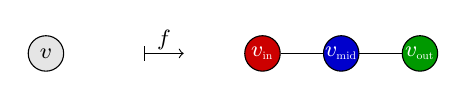
\begin{tikzpicture}[font=\footnotesize, scale=1.0]
\node[draw, fill=gray!20, circle, minimum size=0.45cm, inner sep=0cm] (v) at (0.25,0) {\(v\)};

\draw[|->] (1.5, 0) -- node[above, midway, inner sep=1pt] {\(f\)} (2.0, 0);

\begin{scope}[shift={(4,0)}]
\node[draw, fill=red!80!black, circle, minimum size=0.45cm, inner sep=0cm] (vin) at (-1,0) {\textcolor{white}{\(v_{\raisebox{-0.0ex}{\scalebox{0.5}{in}}}\)}};
\node[draw, fill=blue!80!black, circle, minimum size=0.45cm, inner sep=0cm] (vmid) at (0,0) {\textcolor{white}{\(v_{\raisebox{-0.0ex}{\scalebox{0.5}{mid}}}\)}};
\node[draw, fill=green!60!black, circle, minimum size=0.45cm, inner sep=0cm] (vout) at (1,0) {\textcolor{white}{\(v_{\raisebox{-0.0ex}{\scalebox{0.5}{out}}}\)}};
\draw[] (vin) -- (vmid) -- (vout);
\end{scope}
\end{tikzpicture}
\]

Now \(G\) has a directed Hamiltonian cycle iff \(G'\) has a Hamiltonian cycle.
\begin{itemize}
\item
`\(\Rightarrow\)': 
Suppose \(G\) has a directed Hamiltonian cycle.
Then \(G'\) has an undirected Hamiltonian cycle (same order).
\item
`\(\Leftarrow\)':
Suppose \(G'\) has an undirected Hamiltonian cycle.
must visit nodes either in order \(v_{\text{in}} \to v_{\text{mid}} \to v_{\text{out}}\) or \(v_{\text{out}} \to v_{\text{mid}} \to v_{\text{in}}\).
The \(v_{\text{mid}}\) nodes in the cycle make up a directed Hamiltonian cycle in \(G\), or reverse of one.
\qedhere
\end{itemize}
\end{proof}

\begin{problem}[Traveling Salesman]\label{prob:tsp}
Given a set of \(n\) cities and a pairwise distance function \(d(u,v)\),
is there a tour of length \(\leq D\) that visits each city exactly once and returns to the starting city?
\end{problem}

\begin{claim}\label{claim:ham-cycle-reduces-to-tsp}
\(\text{\hyperref[prob:ham-cycle]{HAM-CYCLE}} \leq_{P} \text{\hyperref[prob:tsp]{TSP}}\).  
\end{claim}
\begin{proof}
Given an instance \(G=(V,E)\) of \nameref{prob:ham-cycle}, create \(n=|V|\) cities with distance function
\[
d(u,v) 
= 
\begin{cases}
1 & \text{if } (u,v) \in E\\
2 & \text{otherwise}
\end{cases}
\]

\textcolor{AccentBlue}{Remark}. 
\hyperref[prob:tsp]{TSP} instance in reduction satisfies \(\triangle\)-inequality:
\(
d(u,v) \leq 2 \leq d(u,w) + d(w,v)
\)
% for all cities \(u,v,w\).

\hyperref[prob:tsp]{TSP} instance has tour of length \(\leq n\) iff \(G\) is Hamiltonian.

\begin{itemize}
\item
`\(\Leftarrow\)': 
If \(G\) has a Hamiltonian cycle, then it defines a tour of length \(n\) in the \hyperref[prob:tsp]{TSP} instance.
\item
`\(\Rightarrow\)':
Suppose there is a tour \(T\) of length \(\leq n\) in the \hyperref[prob:tsp]{TSP} instance.
The length of \(T\) is the sum of \(n\) terms, each of which has cost at least \(1\) (\(1\) or \(2\)).
Since the length of \(T\) is at most \(n\), each term must have cost \(1\).
Thus, each pair of consecutive cities in \(T\) must be connected by an edge in \(G\).
Thus, the order of \(T\) gives a Hamiltonian cycle in \(G\).
\qedhere
\end{itemize}
\end{proof}





\begin{claim}\label{claim:3-sat-reduces-to-dir-ham-cycle}
\(\text{\hyperref[prob:3-sat]{3-SAT}} \leq_{P} \text{\hyperref[prob:dir-ham-cycle]{DIR-HAM-CYCLE}}\).
\end{claim}

% \begin{proof}
% Given an instance \(\Phi\) of \nameref{prob:3-sat}, we construct an instance of \nameref{prob:dir-ham-cycle} that has a Hamiltonian cycle iff \(\Phi\) is satisfiable.

% \textcolor{AccentBlue}{Construction}.
% Create a graph that has \(2^n\) Hamiltonian cycles which correspond ina natural way to \(2^n\) truth assignments.

% Given \hyperref[prob:3-sat]{3-SAT} instance \(\Phi\) with \(n\) variables and \(k\) clauses,
% \begin{itemize}
%   \item 
%   construct \(G\): 
%   1 bi-directional path (\(3k+3\) nodes) for each variable (\(n\) paths).
%   For left and right endpoints of variable \(x_i\) path, connect them to the left and right endpoints of variable \(x_{i+1}\) path, for \(i=1, \ldots, n-1\) (left to left, left to right, right to left, right to right).
%   Add nodes \(s,t\). 
%   Add directed edges from \(s\) to left and right endpoints of first variable (\(x_1\)) path.
%   Add directed edges from left and right endpoints of last variable (\(x_n\)) path to \(t\).
%   Add a directed edge from \(t\) to \(s\).
%   (so far, \(G\) has \(2^n\) Hamiltonian cycles, one for each truth assignment).
%   \item
%   Traverse path \(i\) from left to right \(\Leftrightarrow\) set variable \(x_i = 1\).
%   \item
%   For each clause \(C_j\), add a node \(C_j\) and 6 directed edges
% \end{itemize}

% \medskip

% \textcolor{AccentBlue}{Claim}.
% \(\Phi\) is satisfiable iff \(G\) has a Hamiltonian cycle.

% `\(\Rightarrow\)':
% \begin{itemize}
% \item
% Suppose \nameref{prob:3-sat} instance has satisfying assignment \(x^*\).
% \item
% Then, define Hamiltonian cycle in \(G\) as follows:
% \begin{itemize}
%   \item if \(x^*_i = 1\), traverse row \(i\) from left to right
%   \item if \(x^*_i = 0\), traverse row \(i\) from right to left
%   \item for each clause \(C_j\), we splice \(C_j\) into the tour exactly once: for the literal that sets \(C_j\) to true.
%   There will be at least one row \(i\) in which we are going in ``correct'' direction to splice node \(C_j\) into tour
%   \item (Note we can splice node \(C_j\) into tour only if we have the right direction)
% \end{itemize}
% \end{itemize}

% `\(\Leftarrow\)':
% \begin{itemize}
% \item
% Suppose \(G\) has a Hamiltonian cycle \(H\).
% \item
% If \(H\) enters clause node \(C_j\), it must depart on mate edge.
% \begin{itemize}
%   \item thus, nodes immediately before and after \(C_j\) are connected by an edge \(e\) in \(G\)
%   \item removing \(C_j\) from cycle \(H\), and replacing it with edge \(e\) yields Hamiltonian cycle on \(G \setminus \{ C_j \}\).
% \end{itemize}
% \item
% Continuing in this way, we are left with Hamiltonian cycle \(H'\) in \(G \setminus \{ C_1, \ldots, C_k \}\).
% \item
% Set \(x^*_i = 1\) iff \(H'\) traverses row \(i\) left to right.
% \item
% Since \(H\) visits each clause node \(C_j\), at least one of the paths is traversed in ``correct'' direction, and each clause is satisfied.
% \qedhere
% \end{itemize}
% \end{proof}


\begin{proof}
Let $\Phi$ be a 3-\hyperref[def:CNF]{CNF} formula with \(n\) variables $x_1,\dots,x_n$ and \(k\) clauses $C_1,\dots,C_k$, i.e.,
\[
\Phi 
= \bigwedge_{j=1}^k C_j
= \bigwedge_{j=1}^k (L_{j,1} \vee L_{j,2} \vee L_{j,3}),
\]
where each literal \(L_{j,m}\) is either \(x_i\) or \(\neg x_i\) for some \(i \in \{1,\dots,n\}\).

We construct a directed graph $G$ as follows.

% \paragraph{Variable paths.}
Let $b := 3k+3$.
For each variable $x_i$ construct a directed path
\[
P_i = (v_{i,1}, v_{i,2}, \dots, v_{i,b-1}, v_{i,b})
\]
where for every $q \in \{1,\dots,b-1\}$ we add both directed edges
$(v_{i,q},v_{i,q+1})$ and $(v_{i,q+1},v_{i,q})$.
Let $\ell_i := v_{i,1}$ and $r_i := v_{i,b}$.

For $i=1,\dots,n-1$, add all four directed edges
$\ell_i \to \ell_{i+1}$, $\ell_i \to r_{i+1}$, $r_i \to \ell_{i+1}$,
$r_i \to r_{i+1}$.
Add vertices $s,t$ and directed edges
$s \to \ell_1$, $s \to r_1$, $\ell_n \to t$, $r_n \to t$, and $t \to s$.
Let $G_0$ denote the resulting graph:
\[
\begin{tikzpicture}[
  >={Latex[length=1.35mm, width=0.9mm]},
  v/.style={circle,draw,fill=gray!20,minimum size=3.8mm,inner sep=0pt},
  ed/.style={->,thin},
  lab/.style={font=\footnotesize, outer sep=0pt, inner sep=3pt},
  font=\footnotesize,
  scale=0.8
]

% ---- geometry ----
\def\dx{1.4}
\def\dy{2}

% x-positions (schematic): left block, dots, right block
\coordinate (X0) at (0,0);
\coordinate (X1) at (\dx,0);
\coordinate (X2) at (2*\dx,0);
\coordinate (X3) at (3*\dx,0);
\coordinate (Xd) at (4*\dx,0);   % where \cdots goes
\coordinate (Xr3) at (5*\dx,0);
\coordinate (Xr2) at (6*\dx,0);
\coordinate (Xr1) at (7*\dx,0);
\coordinate (Xr0) at (8*\dx,0);

% y-positions: top row, second row, dots, last row
\coordinate (Y1) at (0,0);
\coordinate (Y2) at (0,-\dy);
\coordinate (Yd) at (0,-2.1*\dy);  % where \vdots goes
\coordinate (Yn) at (0,-3.2*\dy);

% ---- helper macro to draw one schematic row i at y ----
% creates endpoints Li,Ri and a few inner nodes + \cdots
\newcommand{\Row}[2]{% #1 = row name (1,2,n), #2 = y
  % endpoints
  \node[v] (L#1) at ($(X0)+(0,#2)$) {$\ell_{#1}$};
  \node[v] (R#1) at ($(Xr0)+(0,#2)$) {$r_{#1}$};

  % left few nodes
  \node[v] (A#1) at ($(X1)+(0,#2)$) {};
  \node[v] (B#1) at ($(X2)+(0,#2)$) {};
  \node[v] (C#1) at ($(X3)+(0,#2)$) {};

  % right few nodes
  \node[v] (D#1) at ($(Xr3)+(0,#2)$) {};
  \node[v] (E#1) at ($(Xr2)+(0,#2)$) {};
  \node[v] (F#1) at ($(Xr1)+(0,#2)$) {};

  % horizontal dots
  \node at ($(Xd)+(0,#2)$) {$\cdots$};

  % bidirectional edges (left block)
  \draw[<->, thin] (L#1) -- (A#1);
  \draw[<->, thin] (A#1) -- (B#1);
  \draw[<->, thin] (B#1) -- (C#1);

  % connect to dots region and out again (schematic connectors)
  \draw[<-, thin] (C#1) -- ($(Xd)+(-0.55, #2)$);
  \draw[->, thin] ($(Xd)+(0.55, #2)$) -- (D#1);

  % bidirectional edges (right block)
  \draw[<->, thin] (D#1) -- (E#1);
  \draw[<->, thin] (E#1) -- (F#1);
  \draw[<->, thin] (F#1) -- (R#1);
}


% draw rows x1, x2, xn 
\Row{1}{0}
\Row{2}{-\dy}
\Row{n}{-3*\dy}

% row labels
\node[lab,left=15pt] at (L1.west) {$P_1$:};
\node[lab,left=15pt] at (L2.west) {$P_2$:};
\node[lab,left=15pt] at (Ln.west) {$P_n$:};

% G_0 label
\node[draw, rectangle, rounded corners, align=left, text width=3.3cm, inner sep=2pt] at (7.8*\dx, 1.1*\dy) {\(G_0\): Hamiltonian cycles correspond to the \(2^n\) possible truth assignments};

% s,t 
\node[v] (s) at ($(Xd)+(0,1.25*\dy)$) {$s$};
\node[v] (t) at ($(Xd)+(0,-4.25*\dy)$) {$t$};


% show all 4 edges between x1 and x2
\draw[->, thin] (L1) -- (L2);
\draw[->, thin] (L1.south east) -- (R2.north west);
\draw[->, thin] (R1.south west) -- (L2.north east);
\draw[->, thin] (R1) -- (R2);


\draw[-, thin] (L2.south) -- ($(L2.south)!0.34!($(L2.south) + (0,-\dy)$)$);
\draw[-, thin] (L2.south east) -- ($(L2.south east)!0.34!($(R2) + (0,-\dy)$)$);
\draw[-, thin] (R2.south west) -- ($(R2.south west)!0.34!($(L2) + (0,-\dy)$)$);
\draw[-, thin] (R2.south) -- ($(R2.south)!0.34!($(R2.south) + (0,-\dy)$)$);

% vertical dots between rows
\node at ($(Xr0)+(0,-1.9*\dy)$) {$\vdots$};
\node at ($(X0)+(0,-1.9*\dy)$) {$\vdots$};
\node at ($(Xd)+(0,-1.9*\dy)$) {$\vdots$};

\draw[->, thin] ($(Ln.north)!0.34!($(Ln.north) + (0,\dy)$)$) -- (Ln.north);
\draw[->, thin] ($(Rn.north west)!0.34!($(Ln) + (0,\dy)$)$) -- (Rn.north west);
\draw[->, thin] ($(Ln.north east)!0.34!($(Rn) + (0,\dy)$)$) -- (Ln.north east);
\draw[->, thin] ($(Rn.north)!0.34!($(Rn.north) + (0,\dy)$)$) -- (Rn.north);


% ---- edges from s to first row endpoints ----
\draw[->, thin] (s) -- (L1);
\draw[->, thin] (s) -- (R1);

% ---- edges from last row endpoints to t ----
\draw[->, thin] (Ln) -- (t);
\draw[->, thin] (Rn) -- (t);

% ---- edge t -> s ----
\coordinate (svirtual) at ($(t)+(-4,0.2)$);
\draw[->, thin, bend left=30, dashed] (t) to (svirtual) node[above] {to $s$ ...};

% ---- length marker (schematic) ----
\draw[|-|] ($(Ln)+(-0.1,-3.5)$) -- node[below] {$3k+3$} ($(Rn)+(0.1,-3.5)$);

\end{tikzpicture}
\]
$G_0$ has exactly $2^n$ different Hamiltonian cycles, corresponding to the $n$ independent choices of direction for traversing each path $P_i$.

This naturally models the $n$ independent choices of how to set each variable \(x_1, \dots, x_n\) to \texttt{true} or \texttt{false},
and hence the $2^n$ truth assignments.
Thus, we identify each Hamiltonian cycle $H_0$ in $G_0$ uniquely with a truth assignment $a$ as follows:
If $H_0$ traverses path $P_i$ from left to right, set $a(x_i) := 1$;
if $H_0$ traverses path $P_i$ from right to left, set $a(x_i) := 0$.


\begin{lemma*}\label{lem:choice_of_directions_induces_ham_cycle}
Every Hamiltonian cycle in $G_0$ traverses each path $P_i$ entirely
from $\ell_i$ to $r_i$ or entirely from $r_i$ to $\ell_i$.
Conversely, every choice of directions for $P_1,\dots,P_n$
induces a unique Hamiltonian cycle in $G_0$.
\end{lemma*}
\begin{proof}
Since the only edges incident to internal vertices of $P_i$ are the two path edges
to their predecessor/successor, a Hamiltonian cycle cannot enter or leave $P_i$
at an internal vertex.
Hence it must enter at one endpoint and leave at the other, traversing $P_i$
completely in one direction.
The endpoint connections guarantee that all $2^n$ direction choices are feasible and independent.
\end{proof}



Next we add nodes to model the constraints imposed by the clauses of \(\Phi\).

% \paragraph{Clause nodes.}
For each clause $C_j$, add a vertex $c_j$.
We reserve positions $3j$ and $3j+1$ on each path $P_i$ for clause $C_j$.
For each literal $L \in C_j$:
\begin{itemize}
\item if $L = x_i$, add edges $(v_{i,3j},c_j)$ and $(c_j,v_{i,3j+1})$
\item if $L = \neg x_i$, add edges $(v_{i,3j+1},c_j)$ and $(c_j,v_{i,3j})$
\end{itemize}

This completes the construction of $G$.

\begin{lemma*}[Splicing]\label{lem:splicing_clause_into_ham_cycle}
Let $H$ be a Hamiltonian cycle containing a directed edge $p \to q$.
If $G$ contains edges $p \to c_j$ and $c_j \to q$, then replacing
$p \to q$ in $H$ by $p \to c_j \to q$ yields another Hamiltonian cycle.
\end{lemma*}
\begin{proof}
The replacement preserves indegree and outdegree $1$ at all vertices
and introduces no repetitions.
\end{proof}

Now \(\Phi\) is satisfiable iff \(G\) has a Hamiltonian cycle.
\begin{itemize}
\item
`\(\Rightarrow\)':
Suppose $\Phi$ is satisfiable, and let $a$ be a satisfying assignment.
By the \hyperref[lem:choice_of_directions_induces_ham_cycle]{first Lemma}, $a$ induces a Hamiltonian cycle $H_0$ in $G_0$.

Fix a clause $C_j$.
Choose a literal $L \in C_j$ satisfied by $a$ 
% (it must exist, since $a$ satisfies $\Phi$ iff it satisfies every $C_j$ and $C_j$ is satisfied only if at least one literal in $C_j$ is true).
(at least one must exist by assumption that $\Phi$ is satisfiable).
\begin{itemize}
\item 
If $L=x_i$, 
then $a(x_i)=1$, so $H_0$ traverses $P_i$ left-to-right and in particular uses the edge $v_{i,3j} \to v_{i,3j+1}$.
By construction, $G$ contains edges $v_{i,3j} \to c_j$ and $c_j \to v_{i,3j+1}$, so by
the \hyperref[lem:splicing_clause_into_ham_cycle]{second Lemma} 
we can splice $c_j$ into the tour between $v_{i,3j}$ and $v_{i,3j+1}$.
\item 
If $L=\neg x_i$, 
then $a(x_i)=0$, so $H_0$ traverses $P_i$ right-to-left and in particular uses the edge $v_{i,3j+1} \to v_{i,3j}$.
By construction, $G$ contains edges $v_{i,3j+1} \to c_j$ and $c_j \to v_{i,3j}$, so by
the \hyperref[lem:splicing_clause_into_ham_cycle]{second Lemma} 
we can splice $c_j$ into the tour between $v_{i,3j+1}$ and $v_{i,3j}$.
\end{itemize}
Do this once for each clause $C_j$.
The resulting directed cycle visits every vertex exactly once, hence is a Hamiltonian cycle of $G$.

\item
`\(\Leftarrow\)':
Suppose $G$ has a Hamiltonian cycle $H$.
Fix $j$.
Since $c_j$ has indegree and outdegree $1$ in $H$, the cycle contains a subpath
$p \to c_j \to q$.

Moreover, if $H$ enters $c_j$ from $v_{i,3j}$ then it must leave to $v_{i,3j+1}$:
otherwise $v_{i,3j+1}$ would remain unvisited and would then have only one unvisited 
neighbor $v_{i,3j+2}$ available, so the tour will not be able to visit this node while remaining Hamiltonian.
Symmetrically, if $H$ enters from $v_{i,3j+1}$ then it must leave to $v_{i,3j}$.

By construction of $G$, necessarily $(p,q)=(v_{i,3j},v_{i,3j+1})$ for some $i$ (if $c_j$ encodes a
positive occurrence $x_i$) or $(p,q)=(v_{i,3j+1},v_{i,3j})$ (if it encodes a negative occurrence $\neg x_i$).
In either case, the shortcut edge $p \to q$ is a path edge of $P_i$ and hence belongs to $G_0$.
Contract $p \to c_j \to q$ to $p \to q$.
Repeating this for all $j=1,\dots,k$ yields a Hamiltonian cycle $H_0$ of $G_0$.

By the \hyperref[lem:choice_of_directions_induces_ham_cycle]{first Lemma}, $H_0$ induces an assignment $a$ by setting
$a(x_i)=1$ iff $H_0$ traverses $P_i$ left-to-right.
Fix a clause $C_j$.
Since $H$ visits $c_j$, it must splice through $c_j$ using some path $P_i$ in the direction that matches
the corresponding literal in $C_j$; hence that literal is true under $a$.
Therefore every clause is satisfied by $a$, so $\Phi$ is satisfiable.
\end{itemize}

Complexity:
The graph has $O(n \cdot k)$ vertices and edges and is constructible in polynomial time.
\end{proof}












% \clearpage



\subsection{Approximation Algorithms}\label{sec:approximation_algorithms}

We saw all these problems that are NP-complete and reduce one to another.
So they are the same hard.
They appear extremely often in practice.

So how do we cope with NP-completeness?
\begin{itemize}
  \item \textbf{brute-force search}: viable only for small input sizes (e.g. \(n \leq 20\)).
  \item \textbf{heuristics}: strategy for producing a valid solution, but no guarantee on how close is to optimal
  \item \textbf{general search algorithms}: powerful techniques for solving general combinatorial optimization problems:
  \begin{itemize}
  \item branch-and-bound: breaking problem down into smaller subproblem and using a bounding function % https://en.wikipedia.org/wiki/Branch_and_bound
  \item metropolis-hastings: Markov chain Monte Carlo method for obtaining a sequence of random samples from a probability distribution from which direct sampling is difficult % https://en.wikipedia.org/wiki/Metropolis–Hastings_algorithm
  \item simulated annealing: models the physical process of heating a material and then slowly lowering the temperature to decrease defects, thus minimizing the system energy % https://www.mathworks.com/help/gads/what-is-simulated-annealing.html
  \item genetic algorithms: metaheuristic used to generate high-quality solutions to optimization and search problems via biologically inspired operators such as selection, crossover, and mutation % https://en.wikipedia.org/wiki/Genetic_algorithm
  \end{itemize}
  performance varies considerably from problem to problem and instance to instance
  \item \textbf{approximation algorithms}: algorithm that runs in polynomial time and produces a solution that is guaranteed to be within some factor of the optimal solution
\end{itemize}

\medskip

\textcolor{AccentBlue}{Performance Bounds}:
\begin{itemize}
  \item most NP-complete problems states as decision problems (because of theoretical resons involving complexity) 
  \item they are natural optimization problems, e.g. 
  \begin{itemize}
  \item \nameref{prob:vertex-cover}: find vertex cover of minimum size
  \item \nameref{prob:clique}: find the clique of maximum size
  \end{itemize}
  \item an approximation algorithm returns a legitimate answer, but not necessarily one of optimal size
\end{itemize}

\medskip

\textcolor{AccentBlue}{Measuring how good an approximation algorithm is}:
\begin{itemize}
  \item define the \emph{performance ratio} of an approximation
  \item given an instance \(I\) of our problem,
  \begin{itemize}
    \item let \(C(I)\) be the cost of solution produced by the approximation algorithm
    \item let \(C^*(I)\) be the cost of optimal solution
  \end{itemize}
  \item for a \emph{minimization problem}: \(C(I) / C^*(I) \geq 1\)
  \item for a \emph{maximization problem}: \(C^*(I) / C(I) \geq 1\)
\end{itemize}


\begin{definition}[Performance Ratio Bound]\label{def:performance_ratio_bound}
We say that an approximation algorithm achieves performance ratio bound \(\rho(n)\) if
\begin{equation}\label{eq:performance_ratio}
\max_I \left(\frac{C(I)}{C^*(I)}, \frac{C^*(I)}{C(I)}\right) \leq \rho(n)
\end{equation}
for all instances \(I\) of size \(|I| = n\) of the problem.
Note that \(\rho(n) \geq 1\) with equality iff the approximate solution is the true optimal solution.
\end{definition}
The \nameref{def:performance_ratio_bound} is an upper bound for the worst-case performance.


\medskip 

\hl{NP-complete problems are equivalent with respect to complexity, but their approximability varies considerably}.
\begin{itemize}
  \item some problems are \emph{inapproximable}: no polynomial-time algorithm achieves a ratio bound \(< \infty\) unless P=NP
  \item some can be approximated, but the ratio bound is a function of \(n\) (e.g. \nameref{prob:set-cover} can be approximated within a factor \(O(\log n)\))
  \item some can be approximated and the ratio bound is constant (e.g. \nameref{prob:vertex-cover} can be approximated within a factor \(2\))
  \item some can be approximated arbitrarily well (e.g. \hyperref[prob:knapsack]{Knapsack})
  \begin{itemize}
    \item user provides a parameter \(\epsilon > 0\) and the algorithm achieves a ratio bound \(1 + \epsilon\)
    \item as \(\epsilon\) approaches \(0\), the running time gets worse
    \item if it runs in polynomial time for any fixed \(\epsilon\), it is called a \emph{polynomial-time approximation scheme} (PTAS)
  \end{itemize}
\end{itemize}









\subsubsection{Vertex Cover}\label{sec:vertex_cover_approximation}
\nameref{prob:vertex-cover} has an approximation algorithm with ratio bound \(\rho(n) = 2\).

\begin{algorithm}[h]
\caption{2-for-1 heuristic for \nameref{prob:vertex-cover}}
\label{alg:vc-2-approx}
\begin{algorithmic}[1]
\Function{VC-2-Approx}{$G=(V,E)$}
  \State $T \gets \emptyset$
  \While{$E \neq \emptyset$}
    \State Select an arbitrary edge $(u,v)$ from $E$ \label{line:vc-2-approx-select-edge}
    \State $T \gets T \cup \{u,v\}$ \Comment{add both endpoints to cover}
    \State Remove from $E$ all edges incident to either $u$ or $v$
  \EndWhile
  \State \Return $T$
\EndFunction
\end{algorithmic}
\end{algorithm}

\begin{claim}\label{claim:vc-2-approx-ratio}
\autoref{alg:vc-2-approx} achieves a performance ratio bound of 
\(
\rho(n) = 2
\).
\end{claim}
\begin{proof}
Consider the set \(T\) output by \autoref{alg:vc-2-approx}.
Let \(A\) be the set of edges selected in line \ref{line:vc-2-approx-select-edge}.
\(|T| = 2|A|\) because both endpoints of each edge of \(A\) are added to \(T\).
But also the optimal solution \(T^*\) must cover the edges in \(A\), which are non-adjacent.
Thus, \(|T^*| \geq |A|\).
Therefore,
\(
|T| 
% = 2|A| 
\leq 2|T^*| 
% \Rightarrow
% \frac{|T|}{|T^*|} \leq 2
\).
\end{proof}

\begin{algorithm}[h]
\caption{Greedy heuristic for \nameref{prob:vertex-cover}}
\label{alg:vc-greedy-approx}
\begin{algorithmic}[1]
\Function{VC-Greedy-Approx}{$G=(V,E)$}
  \State $T \gets \emptyset$
  \While{$E \neq \emptyset$}
    \State Select the vertex \(u\) of maximum degree in \(G\)
    \State $T \gets T \cup \{u\}$ \Comment{add vertex to cover}
    \State Remove from $E$ all edges incident to $u$
  \EndWhile
  \State \Return $T$
\EndFunction
\end{algorithmic}
\end{algorithm}

The greedy heuristic (\autoref{alg:vc-greedy-approx}) does not achieve a constant performance bound, but merely one of \(\Theta(\log n)\).
Nevertheless, experimental studies show that it often works quite well in practice, and for ``typical'' graphs, it will perform better than the 2-for-1 heuristic (\autoref{alg:vc-2-approx}).





\subsubsection{Independent Set}\label{sec:independent_set_approximation}
Unfortunately, approximation factors are not preserved by our transformations.

\begin{claim}\label{claim:is-2-for-1-heuristic-factor}
If we apply the \autoref{alg:vc-2-approx} to find an \nameref{prob:independent-set} of maximum size, the performance ratio is
\[
\rho(n, k) = \frac{n - k}{n - 2k}
\]
which can be arbitrarily large (e.g. for \(k = (n-1)/2\), \(\rho(n, k) = (n + 1)/2\)).
\end{claim}
\begin{proof}
We know from \autoref{lem:clique_independent_vc} that \(V'\) is a \nameref{prob:vertex-cover} for \(G\) iff \(V \setminus V'\) is a \nameref{prob:independent-set} for \(G\).
Let \(T^*\) be an minimum (i.e. optimal) \nameref{prob:vertex-cover} of size \(|T^*| = k\).
Then \(S^* = V \setminus T^*\) is a maximum (i.e. optimal) \nameref{prob:independent-set} of size \(|S^*| = n - k\).
\autoref{alg:vc-2-approx} returns a \nameref{prob:vertex-cover} \(T\) with size \(|T| \leq 2k\) (\autoref{claim:vc-2-approx-ratio}).
Thus \(S = V \setminus T\) is an \nameref{prob:independent-set} of size \(|S| \geq n - 2k\).
The performance ratio is therefore
\(\frac{|S^*|}{|S|} = \frac{n - k}{|S|} \leq \frac{n - k}{n - 2k}\).
% \[
% \begin{verticalhack}
%   \frac{|S^*|}{|S|}
%   =
%   \frac{n - k}{|S|}
%   \leq
%   \frac{n - k}{n - 2k}
% \end{verticalhack}
% \qedhere
% \]
\end{proof}

\subsubsection{Traveling Salesman Problem}\label{sec:tsp_approximation}

\autoref{prob:tsp} was formulated in terms of cities and distances, now we reformulate it in terms of graphs:
\begin{problem}[TSP]\label{prob:graph-tsp}
Given a \emph{complete undirected graph} \(G = (V,E)\) with non-negative edge weights \(w(u,v)\), find a cycle that visits all vertices and has minimum cost.
\end{problem}

Often edge weights satisfy the \(\triangle\)-inequality:
\(
w(u,v) \leq w(u,x) + w(x,v)
\)
\begin{itemize}
\item euclidian distance
\item shortest path in a graph
\end{itemize}

\medskip 

When cost function satisfies \(\triangle\)-inequality, there is an approximation algorithm for \nameref{prob:graph-tsp} with a ratio bound of \(\rho(n) = 2\).

\begin{observation}\label{obs:tsp-geq-mst}
A \nameref{prob:graph-tsp} with one edge removed is just a spanning tree (not necessarily minimum).
%
Thus, cost min \nameref{prob:graph-tsp} tour \(\geq\) cost \nameref{def:mst}.
\end{observation}



\textcolor{AccentBlue}{Idea}:
\begin{itemize}
  \item compute a \nameref{def:mst} \(T\) of \(G\) efficiently, e.g. using \nameref{alg:kruskal}
  \item find some way to convert the \nameref{def:mst} \(T\) into a \nameref{prob:graph-tsp} tour \(H\) while increasing its cost by a constant factor
\end{itemize}

\begin{remark}
  \begin{itemize}
    \item given a free tree, there is a tour of the tree called a \emph{twice around tour} that traverses the edges of the tree twice, once in each direction
    \item this path is not simple, because it revisits vertices, but we can make it simple by \emph{short-cutting}, i.e. skipping over already visited vertices
    \item the order in which vertices are visited using short-cuts is a \emph{preorder traversal} (see \href{https://fabianbosshard.github.io/usi-informatics-course-summaries/usi-algorithms-and-data-structures-summary.pdf}{Algorithms \& Data Structures}, chapter `Binary Search Trees') of the \nameref{def:mst} \(T\)
    \item the triangle inequality assures that the path length will not increase when we take short-cuts
    \item in fact, any subsequence of the twice-around tour which visits each vertex exactly once will suffice (not necessarily in preorder)
    \qedhere
  \end{itemize}
\end{remark}

\begin{algorithm}[h]
\caption{Approximation for \nameref{prob:graph-tsp}}
\label{alg:tsp-approx}
\begin{algorithmic}[1]
\Function{TSP-Approx}{$G=(V,E)$}
  \State \(T \gets \text{MST}(G)\) \label{line:mst-calc}\Comment{e.g. using \nameref{alg:kruskal}}
  \State \(r \gets\) arbitrary root of \(T\)
  \State \(H \gets\) list of vertices visited by a preorder walk of \(T\) starting at \(r\)
  \State \Return \(H\)
\EndFunction
\end{algorithmic}
\end{algorithm}

\begin{claim}\label{claim:tsp-approx-ratio}
\autoref{alg:tsp-approx} achieves a performance ratio bound of 
\(
\rho(n) = 2
\).
\end{claim}
\begin{proof}
Let \(H^*\) be an optimal \nameref{prob:graph-tsp} tour and \(H\) be the tour returned by \autoref{alg:tsp-approx}.
Let \(T\) be the \nameref{def:mst} computed in line \ref{line:mst-calc}.
By \autoref{obs:tsp-geq-mst}, \(W(T) \leq W(H^*)\).
The twice around tour of \(T\) has cost \(2 \cdot W(T)\).
By the triangle inequality, short-cuts do not increase the cost of a tour, i.e. \(W(H) \leq 2 \cdot W(T)\).
Thus, \(W(H) \leq 2 \cdot W(T) \leq 2 \cdot W(H^*) 
\Rightarrow
\frac{W(H)}{W(H^*)} \leq 2\).
\end{proof}



\subsubsection{Set Cover}\label{sec:set_cover_approximation}

\nameref{prob:set-cover} can be generalized where each set \(S_i\) has a positive cost \(w_i\)
and we want to compute the set cover of minimum total weight.
\autoref{alg:set-cover-greedy-approx} can be generalized to this too.

The \nameref{alg:vc-2-approx} relies on the fact that each element (each edge) appears in exactly two sets (one for each endpoint).
This is not true for \nameref{prob:set-cover}\textcolor{red}{!}

\hl[2]{widely believed, there is no constant factor approximation for \nameref{prob:set-cover}}.



\begin{algorithm}[h]
\caption{Greedy heuristic for \nameref{prob:set-cover}}
\label{alg:set-cover-greedy-approx}
\begin{algorithmic}[1]
\Function{SC-Greedy-Approx}{$U, F = \{S_1, \ldots, S_n\}$}
  \State \(X \gets U\) \Comment{uncovered elements}
  \State \(C \gets \emptyset\) \Comment{sets in the cover}
  \While{\(X \neq \emptyset\)}
    \State Select \(S_i \in F\) that covers the most elements of \(X\)
    \State \(C \gets C \cup \{S_i\}\)
    \State \(X \gets X \setminus S_i\)
  \EndWhile
  \State \Return \(C\) \Comment{\autoref{thm:set-cover-greedy-approx-ratio}: \(|C| \le (1 + \ln |U|) \cdot |C^*|\)}
\EndFunction
\end{algorithmic}
\end{algorithm}


\autoref{alg:set-cover-greedy-approx} is a greedy heuristic that at each stage selects the set that covers the greatest number of uncovered elements.


The \nameref{alg:set-cover-greedy-approx} can be ``fooled'' into picking the wrong set over and over again, as the following example shows.
\begin{example}\label{ex:greedy-can-be-fooled}
Consider the following instance of \nameref{prob:set-cover}:
\[
\begin{tikzpicture}[font=\footnotesize,scale=0.8]

% --- parameters ---
\def\dx{0.60}      % horizontal spacing of elements
\def\r{0.085}      % dot radius

\def\smallsep{0.25}
\def\largesep{0.38}

\pgfmathsetmacro{\rowsep}{2*\largesep+\dx-2*\smallsep}  % vertical spacing of rows

% coordinates
\coordinate (T0) at (0,0);                 % first element in top row
\coordinate (B0) at (0,-\rowsep);          % first element in bottom row
\coordinate (T15) at (15*\dx,0);
\coordinate (B15) at (15*\dx,-\rowsep);

% --- dots (16 per row) ---
\foreach \i in {0,...,15}{
  \fill ($(T0)+(\i*\dx,0)$) circle (\r);
  \fill ($(B0)+(\i*\dx,0)$) circle (\r);
}

% ---  optimal sets s7 and s8 ---
\draw[densely dotted, thick] ($(T0)+(-\largesep,\smallsep)$) rectangle ($(T15)+(\largesep,-\smallsep)$);
\node[anchor=west] at ($(T15)+(\largesep,0)$) {$S_7$};
\draw[densely dotted, thick] ($(B0)+(-\largesep,\smallsep)$) rectangle ($(B15)+(\largesep,-\smallsep)$);
\node[anchor=west] at ($(B15)+(\largesep,0)$) {$S_8$};

% ---  greedy sets s1..s6 ---
% convention: s1..s4 span BOTH rows; s5 only top-left; s6 only bottom-left
% element blocks: 1 | 1 | 2 | 4 | 8  (total 16)
\draw[gray, thick] ($(T0)+(-\smallsep,\largesep)$) rectangle ($(T0)+(\smallsep,-\largesep)$); % s5 (top only, element 0)
\node[above] at ($(T0)+(0,\largesep)$) {$S_5$};
\draw[gray, thick] ($(B0)+(-\smallsep,\largesep)$) rectangle ($(B0)+(\smallsep,-\largesep)$); % s6 (bottom only, element 0)
\node[below] at ($(B0)+(0,-\largesep)$) {$S_6$};
\draw[gray, thick] ($(B0)+(\dx-\smallsep,-\largesep)$) rectangle ($(T0)+(\dx+\smallsep,\largesep)$); % s4 (both rows, element 1)
\node[above] at ($(T0)+(\dx,\largesep)$) {$S_4$};
\draw[gray, thick] ($(B0)+(2*\dx-\smallsep,-\largesep)$) rectangle ($(T0)+(3*\dx+\smallsep,\largesep)$); % s3 (both rows, elements 2..3)
\node[above] at ($(T0)+(3*\dx-\smallsep,\largesep)$) {$S_3$};
\draw[gray, thick] ($(B0)+(4*\dx-\smallsep,-\largesep)$) rectangle ($(T0)+(7*\dx+\smallsep,\largesep)$); % s2 (both rows, elements 4..7)
\node[above] at ($(T0)+(5.5*\dx,\largesep)$) {$S_2$};
\draw[gray, thick] ($(B0)+(8*\dx-\smallsep,-\largesep)$) rectangle ($(T0)+(15*\dx+\smallsep,\largesep)$); % s1 (both rows, elements 8..15)
\node[above] at ($(T0)+(11.5*\dx,\largesep)$) {$S_1$};

\end{tikzpicture}
\]
The optimal set cover consists of sets $S_7$ and $S_8$, each of size $16$, but...
\begin{itemize}
  \item initially the three sets \(S_1, S_7, S_8\) each cover \(16\) elements
  \item if ties are broken in the worst possible way, \autoref{alg:set-cover-greedy-approx} picks~\(S_1\)
  \item now the sets \(S_2, S_7, S_8\) each cover \(8\) of the remaining elements 
  \item again, if we choose poorly, \(S_2\) is chosen
  \item and so on...
  \qedhere
\end{itemize}
\end{example}

We generalize \autoref{ex:greedy-can-be-fooled} to any number of elements that is a power of \(2\).
\begin{itemize}
  \item although there is an optimal solution \(2\) sets, \autoref{alg:set-cover-greedy-approx} will select roughly \(\log m\) sets, where \(m = |U|\) 
  \item thus, the \nameref{alg:set-cover-greedy-approx} achieves an approximation factor of roughly \(\frac{\log m}{2}\) on this example
  \item it is possible to slighlty adjust the example such that there are no ties and yet \autoref{alg:set-cover-greedy-approx} has essentially the same ratio bound
\end{itemize}

\begin{theorem}\label{thm:set-cover-greedy-approx-ratio}
\autoref{alg:set-cover-greedy-approx} achieves an approximation factor of \(1 + \ln m\), where \(m = |U|\) denotes the number of elements to be covered.
\end{theorem}
\begin{proof}%[sketch]
Let \(c = |C^*|\) be the size of an optimal set cover.
At any iteration \(i\) with \(m_{i-1}\) uncovered elements remaining, some optimal set must cover at least \(m_{i-1} / c\) of them (Pigeonhole principle).
Since \autoref{alg:set-cover-greedy-approx} chooses the set covering the maximum number of uncovered elements, it removes at least this many, leaving
\[
m_i 
\le 
m_{i-1} - \frac{m_{i-1}}{c}
=
m_{i-1} \left(1 - \frac{1}{c}\right)
\]
elements uncovered after iteration \(i\). 
Applying this recursively, we obtain
\[
m_i
\le
m \left(1 - \frac{1}{c}\right)^i
\]
where we used \(m_0 = m = |U|\).

Now denote by \(g := |C|\) the number of sets returned by \autoref{alg:set-cover-greedy-approx}
(equivalently, the number of iterations).
Right before the \(g^\text{th}\) iterations of \autoref{alg:set-cover-greedy-approx} we therefore have
\[
m_{g-1} 
\le 
m \left(1 - \frac{1}{c}\right)^{g-1} 
=
m \left(\left(1 - \frac{1}{c}\right)^c\right)^{\frac{g-1}{c}}
\le 
m \left(\frac{1}{\eu}\right)^{\frac{g-1}{c}}
\]
elements uncovered,
where we used \((1 - 1/x)^x \le 1/\eu\).

Since at least one element remains uncovered before the last iteration, i.e. \(m_{g-1} \ge 1\), we have 
\[
1 \leq m \left(\frac{1}{\eu}\right)^{\frac{g-1}{c}}
\quad\Rightarrow\quad
\eu^{\frac{g-1}{c}} \leq m
\quad\Rightarrow\quad
\frac{g-1}{c} \leq \ln m
% \quad\Rightarrow\quad
% g \leq c \ln m + 1
\]
which implies \(g \le c \ln m + 1\).

Therefore, \autoref{alg:set-cover-greedy-approx} returns a \nameref{prob:set-cover} of size at most \(1 + \ln(m) \cdot c\).
Since \(1 + \ln(m) \cdot c \leq (1 + \ln m) \cdot c\), we have \(g \leq (1 + \ln m) \cdot c\), 
establishing the claimed \((1 + \ln m)\)-approximation ratio.
\end{proof}




% Even though the greedy heuristic has this relatively high approximation factor, it tends to perform well in practice.

% – the example in which the approximation bound is Ω(log m) is not typical of set cover instances.

% – Is there is a more sophisticated approximation algorithm that has a better approximation factor?

% Answer: such algorithms exist for special cases of set cover, but for the general problem no significantly better approximation bound is believed to be computable in polynomial time.

% – (Formally, such an algorithm would imply that NP has quasipolynomial time algorithms, and the experts do not believe that this is the case.)



Even though the \nameref{alg:set-cover-greedy-approx} has this relatively high approximation factor, it tends to perform well in practice.
\begin{itemize}
  \item the example in which the approximation bound is \(\Omega(\log m)\) is not typical of \nameref{prob:set-cover} instances
  \item more sophisticated approximation algorithms exist for special cases of \nameref{prob:set-cover}, but for the general problem no significantly better approximation bound is believed to be computable in polynomial time
  \item such an algorithm would imply that NP has quasipolynomial time algorithms (Uriel Feige, 1998), and the experts do not believe that this is the case
\end{itemize}



























































